\directlua{dofile("../extensions/functions.lua")}

%%%%%%%%%%%%%%%%%%%%%%%%%%%%%%%%%%%%%%%%%%%%%%%%%
%%%              Document Class               %%%
%%%%%%%%%%%%%%%%%%%%%%%%%%%%%%%%%%%%%%%%%%%%%%%%%

\documentclass[12pt, a4paper, oneside]{report}
% remove comment, below, to compile only the specified chapter (for draft chapter compilations)
%\includeonly{chapters/introduction/main}

%%%%%%%%%%%%%%%%%%%%%%%%%%%%%%%%%%%%%%%%%%%%%%%%%
%%%   Basic Packages and Package Settings     %%%
%%%%%%%%%%%%%%%%%%%%%%%%%%%%%%%%%%%%%%%%%%%%%%%%%

%\usepackage{luatex85}

\usepackage{float}												% customised float support
\usepackage{fancyhdr}											% improved header and footer support
\usepackage{amssymb}												% American Mathematical Society symbols
\usepackage{amsmath}												% American Mathematical Society environments
\usepackage{makeidx}												% automatic index generation
\usepackage{url}													% URL typesetting
\usepackage{texnames}											% BIBTeX, SliTeX, AMSTeX, PiCTeX and TeXsis logos
\usepackage{verbatim}											% multi-line comments
\usepackage[number=none]{glossary}							% glossary file environments

%%%%%%%%%%%%%%%%%%%%%%%%%%%%%%%%%%%%%%%%%%%%%%%%%
%%%          PDFLaTeX-Specific setup          %%%
%%%%%%%%%%%%%%%%%%%%%%%%%%%%%%%%%%%%%%%%%%%%%%%%%

\newcommand{\noopsort}[1]{}

\usepackage[
	pdftex,															% hyperlinked references for PDF output
	bookmarks=true,												% (option) build bookmarks
	bookmarksnumbered=true										% (option) add section numbers to bookmarks
]{hyperref}

\usepackage{pdfpages}											% required for PDF watermarking
\usepackage{epstopdf}											% automatic conversion of EPS images
\usepackage[pdftex]{thumbpdf}									% thumbnail generation for PDF files
\usepackage{pdflscape}											% required by thumbpdf
\usepackage[all]{hypcap}										% correct PDF figure links to top of image

% setup options for hyperlinks

\hypersetup{
	pdfhighlight=/N,												% (option) no visual cue on clicking link
	pdffitwindow=true,											% (option)
	pdfstartview=Fit,												% (option) fit initial view to page
	plainpages=false,												% (option) prevent hyperref page number changes
	breaklinks=true,												% (option) allow link breaking across lines
	colorlinks=true,												% (option) color link text only (no borders)
	pageanchor=false,												% (option) turns off page referencing for title page
	linkcolor=blue,												% (option) internal link color
	citecolor=blue,												% (option) citation link color
	filecolor=blue,												% (option) file link color
	menucolor=blue,												% (option) Acrobat menu link color
	pagecolor=blue,												% (option) page link color
	urlcolor=blue,													% (option) URL link color
}

% PDF meta-data settings

\hypersetup{
	pdftitle    = {\directlua{value(title)}},
	pdfauthor   = {\directlua{value(author)} <\directlua{value(email)}>},
	pdfsubject  = {Some sort of subject (e.g. Data mining)},
	pdfkeywords = {First keyword, second keyword, third keyword},
}

% force LaTeX-compliant spacing
%\directlua { tex.enableprimitives('',tex.extraprimitives()) }


%\pdfadjustspacing=1

%%%%%%%%%%%%%%%%%%%%%%%%%%%%%%%%%%%%%%%%%%%%%%%%%
%%%                  Lengths                  %%%
%%%%%%%%%%%%%%%%%%%%%%%%%%%%%%%%%%%%%%%%%%%%%%%%%

\setlength{\textwidth}{158mm}
\setlength{\hoffset}{4.5mm}
\setlength{\headheight}{15pt}
\setlength{\unitlength}{1pt}
\setlength{\footnotesep}{5mm}

% ensure PDF is centered in display
\setlength{\hoffset}{-10.5mm}

%%%%%%%%%%%%%%%%%%%%%%%%%%%%%%%%%%%%%%%%%%%%%%%%%
%%%               Line Spacing                %%%
%%%%%%%%%%%%%%%%%%%%%%%%%%%%%%%%%%%%%%%%%%%%%%%%%

\newlength{\originalbaselineskip}
\setlength{\originalbaselineskip}{\baselineskip}
\linespread{1.3}

%%%%%%%%%%%%%%%%%%%%%%%%%%%%%%%%%%%%%%%%%%%%%%%%%
%%%               List Counters               %%%
%%%%%%%%%%%%%%%%%%%%%%%%%%%%%%%%%%%%%%%%%%%%%%%%%

\newcounter{listcount}

%%%%%%%%%%%%%%%%%%%%%%%%%%%%%%%%%%%%%%%%%%%%%%%%%
%%%         Index and Glossary Terms          %%%
%%%%%%%%%%%%%%%%%%%%%%%%%%%%%%%%%%%%%%%%%%%%%%%%%

\renewcommand{\glossaryname}{Acronyms}
\renewcommand{\gloskip}{}
\setlength{\namewidth}{79pt}

\newcommand{\idxbf}[1]{\textbf{\hyperpage{#1}}}

\makeglossary
\makeindex

%%%%%%%%%%%%%%%%%%%%%%%%%%%%%%%%%%%%%%%%%%%%%%%%%
%%%        Figures and Floating Bodies        %%%
%%%%%%%%%%%%%%%%%%%%%%%%%%%%%%%%%%%%%%%%%%%%%%%%%

\renewcommand{\topfraction}{0.9}
\renewcommand{\bottomfraction}{0.0}
\renewcommand{\textfraction}{0.1}
\renewcommand{\floatpagefraction}{0.9}
\setcounter{topnumber}{1}
\setcounter{bottomnumber}{0}
\newfloat{graph}{tbp}{lgf}[chapter]
\floatname{graph}{Graph}
\newfloat{algorithm}{tbp}{loa}[chapter]
\floatname{algorithm}{Algorithm}

% bold float caption numbers and reduced size captions
\makeatletter
\long\def\@makecaption#1#2{%
	\vskip\abovecaptionskip
	\sbox\@tempboxa{{\small{\bf #1:} #2}}%
	\ifdim \wd\@tempboxa >\hsize
		{\small{\bf #1:} #2\par}
	\else
		\hbox to\hsize{\hfil\box\@tempboxa\hfil}%
	\fi
	\vskip\belowcaptionskip
}
\renewcommand\floatc@plain[2]{
	\setbox\@tempboxa\hbox{\small{\bf #1:} #2}%
	\ifdim\wd\@tempboxa>\hsize
		{\small{\bf #1:} #2\par}
	\else
		\hbox to\hsize{\hfil\box\@tempboxa\hfil}\fi}
\makeatother

\newlength{\abovesubfiglabelskip}
\setlength{\abovesubfiglabelskip}{0.5\abovecaptionskip}

\begin{document}

%%%%%%%%%%%%%%%%%%%%%%%%%%%%%%%%%%%%%%%%%%%%%%%%%
%%%             Glossary Acronyms             %%%
%%%%%%%%%%%%%%%%%%%%%%%%%%%%%%%%%%%%%%%%%%%%%%%%%

\newacronym{AI}{Artificial Intelligence}{name=AI, description=Artificial Intelligence}
\newacronym{ANN}{Artificial Neural Network}{name=ANN, description=Artificial Neural Network}
\newacronym{CI}{Computational Intelligence}{name=CI, description=Computational Intelligence}

% and any other acronyms you want to use...

%%%%%%%%%%%%%%%%%%%%%%%%%%%%%%%%%%%%%%%%%%%%%%%%%
%%%           Index Sub-References            %%%
%%%%%%%%%%%%%%%%%%%%%%%%%%%%%%%%%%%%%%%%%%%%%%%%%

\index{AI|see{Artificial Intelligence}}
\index{ANN|see{Artificial Neural Network}}
\index{CI|see{Computational Intelligence}}

%%%%%%%%%%%%%%%%%%%%%%%%%%%%%%%%%%%%%%%%%%%%%%%%%
%%%%%%%%%%%%%%%%%%%%%%%%%%%%%%%%%%%%%%%%%%%%%%%%%


\bibliographystyle{plain}
\bibliography{dissertation}
\begin{document}

\chapter{Technical Background}
\label{chap:third}

For a comprehensive text analysis outcome in this study, emphasizing the context dimension is crucial for effective understanding, interpretation, and validation of results. The primary focus is on employing a text mining approach to contextualize: 1) topics derived from tax-related Twitter messages, 2) the sentiment analysis corpus, and 3) the application of machine learning prediction techniques for hashtag recommendation within the context of a tax authority. The examination of message data reveals limited use of hashtags initially in categorizing messages on Twitter, a prominent social media platform for a government department.

The rapid increase in messages, comments, and replies has surpassed the capacity for manual sorting and tagging, impeding the provision of operational services required by users. Consequently, natural language processing technology has emerged to identify pressing issues reflected by the public, prompting relevant departments to address them promptly.

\section{Research Methodology}

\subsubsection{Data}

Social media data serves as a key source of intelligence derived from the interactive dynamics between governments and citizens. The study, focusing on social media engagement for a revenue authority, specifically targeted tweets related to a tax government department in South Africa. To ensure a comprehensive representation of two-way interactions, Twitter data was exclusively collected from an account associated with the tax revenue authority. This collection comprised two distinct datasets: one encompassing government posts communicating with citizens, and the other capturing users' responses to these government tweets. The data extraction was centered around tweets containing the keyword "sarstax," a brand-established term, facilitating the identification of both the organization's messages and the corresponding engagements from citizens. Notably, despite the organization's early international inception in 2012, a significant shift in Twitter usage occurred around 2018. This approach ensures that the collected data aligns effectively with the study objectives, providing a robust foundation for analyzing social media interactions in the context of a revenue authority.

\begin{table}
\centering
\begin{tabular}{ |c|c|c|c|}
 \hline
 username & name & place &tweet\\
 language & mentions & urls & photos\\
 replies & count & retweets & count\\
 likes & count & hashtags & cashtags\\
 link & retweet & quote & url\\
 video & thumbnail & near & geo\\
 source & user rtid & user rt & retweet id\\
 reply to & retweet date\\
 \hline
 \end{tabular}
\caption{First table.}
\label{tab:table1}
\end{table}

The 2018 year marks the beginning of social media use in the revenue authority resulting in the annual data collected annually from 2018 up to year 2021. Therefore this chapter will provide a validation of two data sets that have emanated from the government tax authority usage of Twitter social media with citizens. 

\begin{itemize}
    \item Section X emanates from the brand, government tweets
    
    \item Section Y emanates from the users, citizens tweets
\end{itemize}

\subsection{Revenue Authority Tweets} 
These are tweets emanating from the revenue government for the four year period, 2018 - 2021 forming a data set of 7 877 without retweets.  However, according figure [] 13 features in the data set are not populated such as geo, quoteURL, source, near which may be important for segmentation and regional view. 

\begin{figure}[h!]
\centering
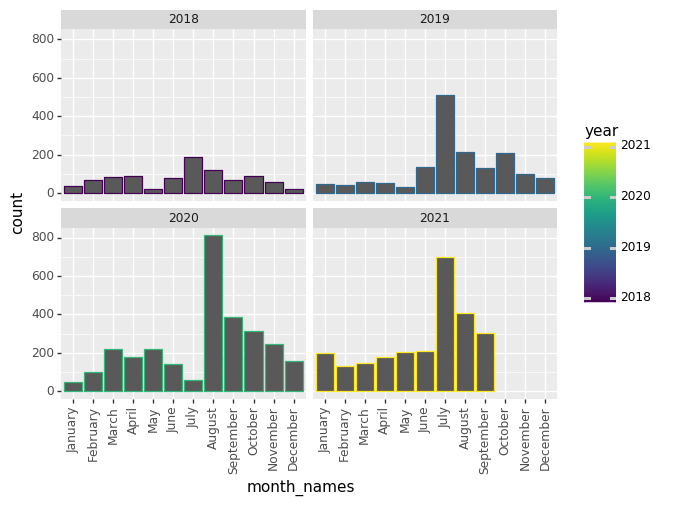
\includegraphics[width=8cm]{postgrad_template 2/Images/Gvt dataset four the four years distribution.png}
\caption{Distribution of GVT Tweets over 4 years.}
\label{fig:figure1}
\end{figure}

Within this dataset, notable aspects of tweet content include 85 percent  lacking hashtags and 26 percent devoid of user mentions. The distribution of tweets per hour reveals a spike during the morning hours, particularly between 4 am and 10 am. Regarding trigrams (3-word sequences), the most frequently repeated phrases include "check profile advice," "send details webmaster," and "send details query."

\subsection{The citizens Tweets} 

The dataset spanning four years comprises 65,919 entries and 34 features, mirroring the number of features in government tweets. Notably, approximately 80 percent of entries lack hashtags. Usernames distribution reveals 11 percent associated with government tweets, followed by 5 percent for civil societies, tax practitioners, and taxpayers each. The most frequently repeated trigrams include "judge bernard ngoepe," "illegal cigarette trade," and "illicit cigarette trade."

\subsection{Tweet Pre-Processing}
The data pre-processing stage entails removing unwanted data features that can make the data noisy for a cleaner data.  In summary the following steps were under taken:

\begin{itemize}
    \item Converting all the tweets into lower case.
\end{itemize}

\begin{itemize}
    \item removal of - duplicated tweets, punctuations, numbers (numeric data); english stop words and domain-related stop words, web links HTML tags(hyperlinks); extra blank spaces; words less than 3 characters;
\end{itemize}

\begin{itemize}
    \item Applied expansion for abbreviations; 
\end{itemize}

\begin{itemize}
    \item "The third step of pre-processing is the normalization of the text under consideration. Normalization is when all the words are brought back to their root level".
\end{itemize}

\begin{itemize}
    \item The second phase involved tokenization, to break larger chunks of data into smaller ones.
\end{itemize}

\subsubsection{Topic Modelling}

In addressing the first part of the RQ1, the age of big data applications and analytics uncovering novel data patterns, this study will employ Latent Dirichlet Allocation (LDA) Topic Model. LDA is an unsupervised machine learning approach designed to extract the meaning from large document corpora, revealing multiple patterns of topics within the text.  According to \cite{blei2011introduction}, Latent Dirichlet Allocation (LDA) is a probabilistic model aimed at uncovering concealed themes within documents, allowing for the inference of hidden topic structures. Alternatively expressed as a soft clustering algorithm, LDA is developed for various applications, including text clustering. In the context of LDA approaches, text clustering implies that each document can encompass multiple scientifically discovered topics, characterized by groups of words that frequently co-occur.
Also \cite{blei2003latent} presents LDA as a generative probabilistic model designed for collections of discrete data. It utilizes a three-level hierarchical Bayesian model to formulate topics, making it applicable to the analysis of social media data. This model illustrates the process by which a specific text corpus might have been generated from certain topics. An illustrative example is [How to identify topics in psychology using topic modeling], showcasing the application of Topic Modeling based on LDA to understand trending topics in psychology research within a large collection of documents.
\cite{mabey2018pyldavis}The exploration and presentation of discovered topics through topic models, allowing for a thorough examination of the relationships between topics and terms in an LDA model, can be facilitated by "PLDAvis," a tool accessible in Python. This tool helps address questions such as: 1) "What is the meaning of each topic?", 2) "How prevalent is each topic?", and 3) "How do the topics relate to each other?"

\subsubsection{Sentiment Analysis}

This subsection also addresses Research Question 2, which explores the evolution of computer-based sentiment analysis. Initially, sentiment analysis was limited to subjective texts available on the web and focused on online product reviews. However, post-2014, the focus shifted to social media texts, particularly from Twitter and Facebook. The significance of incorporating LDA topic modeling alongside qualitative coding for clustering is emphasized.

\cite{liu2010sentiment} describes sentiment analysis involving a series of methods, techniques, and tools for detecting and extracting subjective information, such as opinions and attitudes from language.

The outcomes of sentiment analysis/prediction encompass the labeling of each tweet/retweet based on sentiment polarity. This process enables the calculation/coding of sentiment distribution over time, providing insights into the evolving trends in citizens' behavior in response to government tweets. The final result is a visual representation of monthly sentiment trends, which assists in recognizing significant events/announcements. This strategy is enhanced by insights drawn from Topics/Wordclouds derived through topic modeling. The rationale for integrating both methods is consolidated within the Exploratory Data Analysis (EDA), while the primary focus of the methodology remains on hashtag recommendation.

\subsubsection{Hashtag Recommendation}

\cite{alsini2021hashtag} provides a review of methods for hashtag recommendation on social media platforms, specifically Twitter and Sina Weibo. The authors conduct a systematic literature review to gather research papers on this topic published between 2010 and 2020, discovering that most of the research focuses on the textual content of tweets and that collaborative filtering methods are rarely used in hashtag recommendation. Based on their findings, they propose a taxonomy of hashtag recommendation methods, including text-based methods, hybrid user-based methods, and hybrid miscellaneous methods. They also discuss the challenges and future research directions in this field.

\cite{zhao2016personalized} The paper presents a personalized hashtag recommendation approach using a Latent Dirichlet Allocation (LDA)-based topic model in a microblog environment. The approach combines user profile-based collaborative filtering and LDA-based collaborative filtering to find relevant hashtags for users. The proposed LDA-based model, called Hashtag-LDA, jointly models the relationships between users, hashtags, and words in microblogs. The experimental results on a real Twitter dataset show that the proposed recommendation approach outperforms other related methods and that Hashtag-LDA is effective in finding relevant hashtags.

\cite{godin2013using} this paper introduces an unsupervised and content-based hashtag recommendation method for tweets. The approach utilizes Latent Dirichlet Allocation (LDA) to model the underlying topic assignment of language-classified tweets. The key advantage lies in using a topic distribution for recommending general hashtags. The paper covers related work, details the process of creating a tweet dataset, and outlines the binary classification algorithm used to classify tweets as English or non-English language. The conclusion includes evaluation results and outlines future work. The content-based method employs Latent Dirichlet Allocation (LDA), a hidden generative topic model, enhancing effective categorization and search of tweets while mitigating sparse and noisy tweet content.

\cite{mehrotra2013improving} at the same time addresses challenges in applying topic models, particularly Latent Dirichlet Allocation (LDA), to Twitter content due to the concise and unstructured nature of tweets. The paper investigates various pooling schemes, emphasizing tweet pooling by hashtags, to enhance the quality of topics derived from Twitter data. Through empirical evidence, the authors show that hashtag-based pooling significantly improves topic coherence compared to other schemes and the baseline LDA model. Additionally, the automatic labeling of hashtags further enhances topic quality. The paper offers valuable insights and methods for improving LDA topic models when applied to Twitter content.

This PDF discusses the development of an interactive hashtag recommendation system for social media platforms like Twitter. The system aims to help users enhance their tweets by suggesting relevant hashtags. The system consists of two phases: divergence and convergence. In the divergence phase, the system provides users with related topics based on their input tweet, allowing them to explore novel hashtags. In the convergence phase, the system recommends more accurate hashtags based on the selected topic. The system utilizes natural language processing, topic modeling, and recommendation algorithms to achieve accurate and efficient hashtag recommendations. The system's effectiveness and usability were evaluated through user experiments, with positive results indicating that the interactive hashtag recommendation system provides accurate and helpful hashtags for users.

\cite{alsini2021hashtag} brings a discussion n the development of an interactive hashtag recommendation system for social media platforms like Twitter. The system aims to help users enhance their tweets by suggesting relevant hashtags. The system consists of two phases: divergence and convergence. In the divergence phase, the system provides users with related topics based on their input tweet, allowing them to explore novel hashtags. In the convergence phase, the system recommends more accurate hashtags based on the selected topic. The system utilizes natural language processing, topic modeling, and recommendation algorithms to achieve accurate and efficient hashtag recommendations. The system's effectiveness and usability were evaluated through user experiments, with positive results indicating that the interactive hashtag recommendation system provides accurate and helpful hashtags for users.

\cite{altinel2018semantic} discusses the topic of semantic text classification, which is the task of organizing documents into pre-determined classes using machine learning algorithms. It highlights the importance of capturing the semantics of words and the semantic connections between words, documents, and classes in order to achieve better classification performance. The PDF reviews knowledge-based approaches, such as the use of WordNet, Wiktionary, and Wikipedia as domain knowledge sources, and discusses their advantages over traditional text classification methods. It also explores corpus-based approaches that utilize statistical analysis to discover hidden connections between words in training documents. Additionally, the PDF covers deep learning-based approaches, methods that enhance word/character sequences, and linguistic enriched approaches for semantic text classification. The performance comparison of these approaches is discussed, along with their experimental results and advantages / disadvantages. Overall, the PDF provides a comprehensive overview of semantic text classification and the various approaches used in the field.

Inspired by Community question answering websites that have used both questions text or tags (keywords related to the asked question) topic modelling can summarize and describe content of the question, in this case the extension to understand the context of the tweet for themes and topics of discussion.

\cite{prabha2023question} conducted a study to support that using a text for topic modelling is producing better performance as opposed to using tags when evaluated model using tw metrics namely coherence and perplexity.  In using the users data  (tweets/text), one can determine the hidden information about the user and trending topics across domains.  Hashtags and tags provide context regarding context and semantics.

1. Data Preprocessing:
   - Tokenize the tweets: Split each tweet into individual words or tokens.
   - Remove stop words: Remove common words like "the," "is," "and," etc., as they don't contribute much to the hashtag recommendation process.
   - Stemming/Lemmatization: Reduce words to their base or root form (e.g., "running" becomes "run").
   - Vectorization: Convert the preprocessed tweets into numerical feature vectors using techniques such as TF-IDF.

2. Supervised Model Training:
   - Random Forest Classifier (RFC): Train an RFC model using the preprocessed tweet vectors and their corresponding hashtags as labels.
   - Support Vector Classifier (SVC): Train an SVC model using the same preprocessed tweet vectors and hashtag labels.

3. Unsupervised Topic Model Training:
   - Latent Dirichlet Allocation (LDA): Apply LDA to the preprocessed tweet vectors to discover latent topics within the tweet corpus.

4. Hashtag Recommendation:
   - Given a new tweet, pre-process it and convert it into a feature vector.
   - Use the trained RFC and SVC models to predict the most relevant hashtags for the tweet.
   - Utilize the LDA model to identify the latent topics in the tweet and suggest hashtags related to those topics.
   - The model only Utilized the 7887 tweet messages with identifiable hashtags
This has resulted to recommendation of topics of tweets to organise with an appropriate hashtag for improved user experience that can lead to an efficient two-way communication resulting in organization better services through continuous evidence-based decision making efforts.

\subsubsection{Model Evaluation}

[EVALUATION technique METRIC FOR HASHTAG RECOMMENDATION] The paper examines the assessment of metrics for hashtag recommendation systems, which automatically suggest hashtags to users while composing a tweet. The authors contend that widely used metrics such as hit rate, precision, recall, and F1-score may be insufficient for evaluating hashtag recommendation systems, particularly when the number of ground truth hashtags in tweets varies greatly. They introduce a novel metric termed "hit ratio" to address this issue, considering the varying number of hashtags in the recommended and ground truth sets. The hit ratio is computed as the ratio of matching hashtags over the minimum value between the number of recommended hashtags and the number of ground truth hashtags. The authors compare the hit ratio with traditional evaluation metrics, illustrating its utility through hypothetical scenarios and real-world applications. They assert that the hit ratio offers a more meaningful metric than traditional measures for the evaluation of hashtag recommendation systems.

Some of the evaluation metrics which can be used both for supervised and unsupervised techniques:

\begin{itemize}
    \item Jaccard Score: Calculates the Jaccard similarity score between the predicted hashtags and the actual hashtags for a set of test tweets. Jaccard score measures the similarity between two sets of hashtags.\\
\end{itemize}
\begin{itemize}
    \item Dummy Classifier: Build a dummy classifier to predict whether a tweet is  using the pre-processed tweet vectors for an appropriate hashtag.
\end{itemize}

\begin{itemize}
    \item to iterate and fine-tune the models and evaluation metrics based on the specific characteristics of your tweet dataset and the desired performance.
\end{itemize}
\begin{itemize}
    \item In order to evaluate the text classification supervised models in Topic Modelling unsupervised method to determine their effectiveness in analyzing short text data.   The topic modelling evaluation method is based on "the understandability of extracted topics (topic quality) besides the topic performance and accuracy by applying common standard metrics that apply to the TM domain such as recall, precision, F-score, and topic coherence".
\end{itemize}


\subsubsection{Conclusion}

In conclusion the research methodology has emphasized the importance of understanding the context and domain-specific requirements when selecting and evaluating the algorithms for hashtag recommendation. By considering the unique characteristics of Twitter or the government department's data collection efforts, the researcher has streamlined the methodology to suit the specific needs and challenges of the government environment.
In summary, the research methodology presented in this chapter provides a robust framework for text mining and production techniques aimed at recommending hashtag tags. By combining supervised and unsupervised algorithms, we have demonstrated the potential for enhancing the accuracy and efficiency of hashtag recommendation processes for Twitter or a government department involved in data collection and analysis. This methodology serves as a foundation for the subsequent stages of our research, enabling us to delve deeper into the implementation and evaluation of these techniques and ultimately contribute to the advancements in the field of text mining and recommendation systems."

\bibliographystyle{plain}
\bibliography{dissertation}

\end{document}








%%%%%%%%%%%%%%%%%%%%%%%%%%%%%%%%%%%%%%%%%%%%%%%%%
%%%%%%%%%%%%%%%%%%%%%%%%%%%%%%%%%%%%%%%%%%%%%%%%%

\hypersetup{pageanchor=true}									% (option) turn page referencing back on for chapters

\pagestyle{fancy}
\fancypagestyle{headings}{
	\fancyhead[RO,LE]{\thepage}
	\fancyhead[LO]{\sf\nouppercase{\leftmark}}
	\fancyhead[RE]{\sf\nouppercase{\rightmark}}
	\fancyfoot{}
	\renewcommand{\headrulewidth}{0.4pt}
}

\directlua{input_all(main_includes)}

\chapter{The First Chapter}
\label{chap:first}
\begin{document}

\chapter{Thew Exploratory Data Analysis}
\label{chap:chapter4}

\section{Introduction}

The use of social media technology tools in government can be effective to  achieve digital footprint to streamline the delivery of services and user engagement.  The research study initiates by exploratory analysis of Twitter data set generated by users for a period from 2016 to 2021, indirectly generating big data and through analytics capabilities to uncover hidden patterns from historical data to aid future decision making.   The outcomes of the chapter is mainly comprised of firstly descriptive aspects an analytic process to uncover twitter behavioural characteristics to address first RQ1. This is done by measuring engagement between government and public users on twitter, by exploring features and trends of behaviour over time.  Secondly to answer the RQ2, with further reviewing overall trending topics for the four year summarised to provide insights of past conversations and determined sentiments ratings as results from text mining of a tax government department in analytic outcomes.  Overall outcome of the chapter will guide necessary machine learning use (RQ3) for future solution based on hindsight from data insight in understanding engagement, behaviour characteristics for participation for effective use of Twitter by the government agency to make a difference.\\

\section{User: Government Agency}

With the government agency as Twitter user with an interaction with citizens with rigour from 2018 to 2021 has accumulated in 7 896 messages indicating a strategy of customer service agency, a transactional tactic based on a dedicated social media team that can offer individualised responses as shown by the analysis.

The exploration of social media data through analytics is an important step to understand engagement behaviour between users as contributors to the data.  This data has been acted upon for exploring data characteristics aspects and features such as likes, retweeted messages, replies messages while providing understanding at a glance engagement aspects up to the topics and overall sentiments.  Therefore, the framework that has guided the research methods for the study data analysis and experiment needed is the ground theory approach guided by the exploratory analysis results.  This approach has discovered that users tweets have little usage of hashtags, thus resulting in a hashtag recommendation system to optimize effective use of social media for tweets for the government department under a decade of using twitter.\\
By looking at the average impressions of the number of times a tweet has been seen by users on the social media platform," to track the reach and engagements of tweets to determine the impact of their content on Twitter.\\
The user activity in terms of time is at the highest early hours of the morning, from 05h00 until midday, while seems to stop at about 9pm.\\
The user data does not contain any retweets.  Hence any other duplicates were removed for an amount of 7 867 tweets originating from the government agency.\\
Overall, about 26 percent (2 059)of tweets have not been replied to, meaning the more than 70 percent of tweets have been replied to by the government agency in relation to its social media policy.  This implies a customer service Twitter Strategy for a government department with dedicated staff responding to tweets with assistance of knowledge experts inside the organisation.\\

\begin{itemize}
    \item User participation (Time and Months)
\end{itemize}

Average impressions per tweet by hour tweeted:
----------------------------------------------
12 - 13 : 0.0 = 487 tweets\\
11 - 12 : 0.0 = 675 tweets\\
 8 - 9  : 0.0 = 707 tweets\\
 7 - 8  : 0.0 = 826 tweets\\
 6 - 7  : 0.0 = 957 tweets\\
 5 - 6  : 0.0 = 1361 tweets\\
14 - 15 : 0.0 = 126 tweets\\
10 - 11 : 0.0 = 730 tweets\\
 4 - 5  : 0.0 = 681 tweets\\
13 - 14 : 0.0 = 252 tweets\\
 9 - 10 : 0.0 = 793 tweets\\
 3 - 4  : 0.0 = 111 tweets\\
15 - 16 : 0.0 = 53 tweets\\
16 - 17 : 0.0 = 23 tweets\\
18 - 19 : 0.0 = 4  tweets\\
20 - 21 : 0.0 = 3  tweets\\
 2 - 3  : 0.0 = 49 tweets\\
 1 - 2  : 0.0 = 20 tweets\\
17 - 18 : 0.0 = 18 tweets\\
19 - 20 : 0.0 = 1  tweets\\

Time trends show an urgency dedicated to customer service department strategy with engagement of more than 12 hours in a day.   The first year for the user (department) Twitter full implementation of social media strategy in 2016 as evidently shown in fig 1, since then  there has been a sturdy increase in its usage, in all the 4 yeas shown the most busiest months are mainly July, August, September and October.  These are months associated with individual filing of returns for the tax Season which starts in July.\\

\begin{figure}
      \centering
	    \begin{subfigure}{0.3\linewidth}
		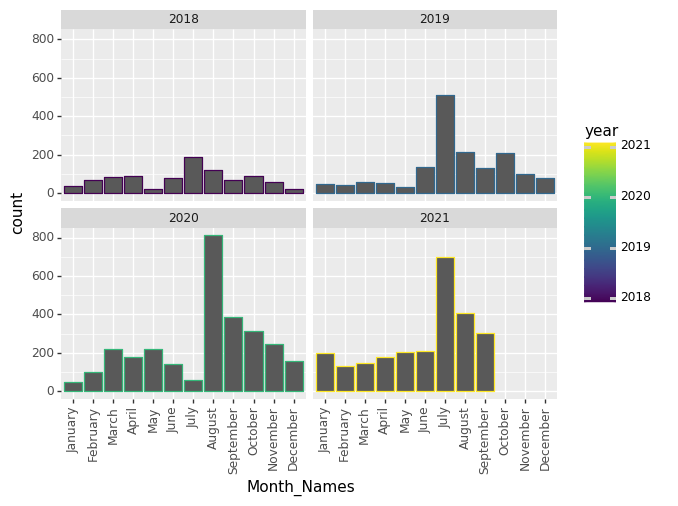
\includegraphics[width=\linewidth]{Users Month Names.png}
		\caption{Monthly engagements}
		\label{fig: Monthly Breakdown for engagement}
	   \end{subfigure}
	   \begin{subfigure}{0.3\linewidth}
		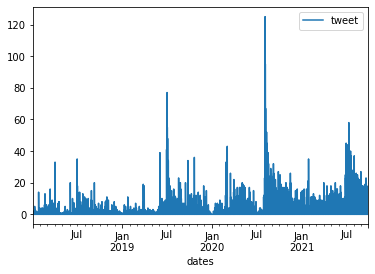
\includegraphics[width=\linewidth]{User 1 Minute Count.png}
		\caption{Time trends outputs}
		\label{fig:Breakdown of time trends by minute}
	    \end{subfigure}
	   \vfill
	 \caption{Time Comparison Monthly vs. Minutes in user engagement.}
\end{figure}

\begin{itemize}
    \item Hashtag Analysis
\end{itemize}

Another aspect to consider is hashtag use, in total for the 7 867 unique records of tweets, only 729 tweets have some representation of hashtags, meaning that 91 percent of tweets do not have any hashtags.  As a result of peaks in Twitter during the tax season for submission of returns by individuals, despite less than 15 percent of tweets use hashtags. The most popular used hashtags are in relation to the context of the filing season, YourTaxMatters(219), SARSTaxTips19(48), TaxSeason2018 (26), SARSRevenueAnnouncement(24), BRICS10Customs(22).\\

\begin{figure}
    \centering
    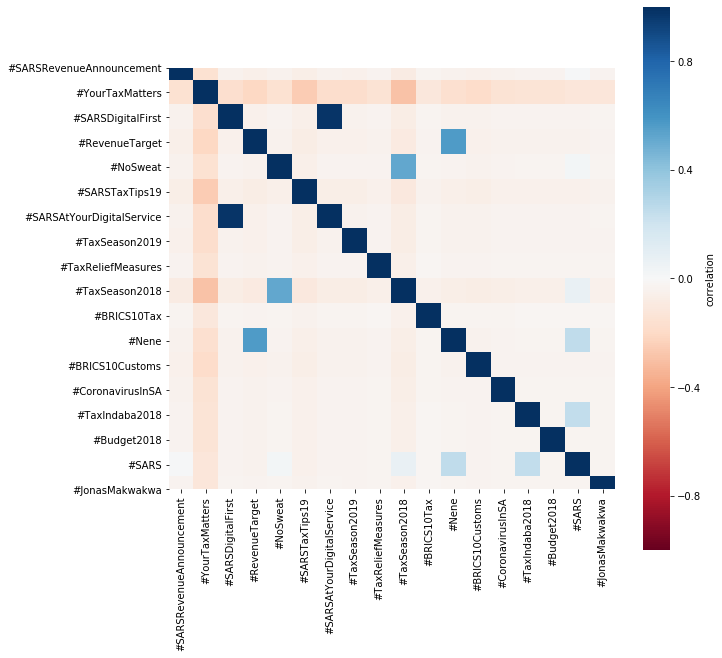
\includegraphics[width=0.1\linewidth]{User Hashtag Correlation.png}
    \caption{Hashtag correlation output}
    \label{fig:Hashtag correlation for government user}
\end{figure}

The correlation matrix shows the following relationship between the most used hashtags
\begin{itemize}
    \item SARSTaxTips19 has a strong positive relationship with YourTaxMatters.  
    \item TaxSeason2018 has a negative relationship with YourTaxMatters.  
    \item TaxSeason2018 has a strong positive relationship with Nosweat
    \item  Nene has a positive relationship with RevenueTarget
    \item  Nene has a positive relationship with SARS 
\end{itemize}

This could mean sending of tax tips in 2019 tax year were helpful for the tax season activities.  The 2018 tax season was not so instrumental.  However, at the same time for the 2018 with a strong support of no sweat campaigns.  Nene had a favourable revenue announcement for tax collection and with SARS in general.

\begin{figure}
      \centering
	    \begin{subfigure}{0.3\linewidth}
		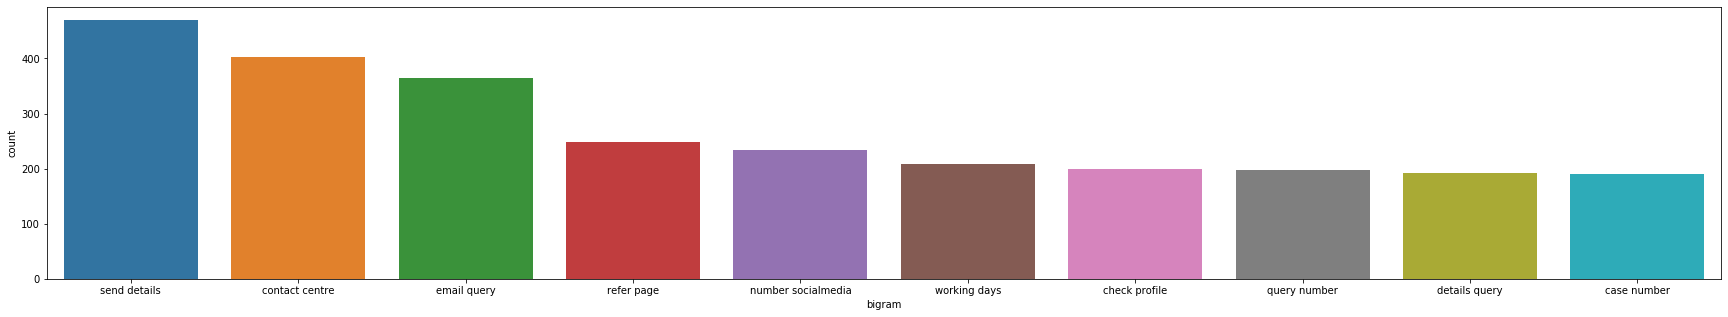
\includegraphics[width=\linewidth]{Bigrams User Data.png}
		\caption{Bi-Grams outputs for government User}
		\label{fig: Associated Bi-Grams Outputs}
	   \end{subfigure}
	   \begin{subfigure}{0.3\linewidth}
		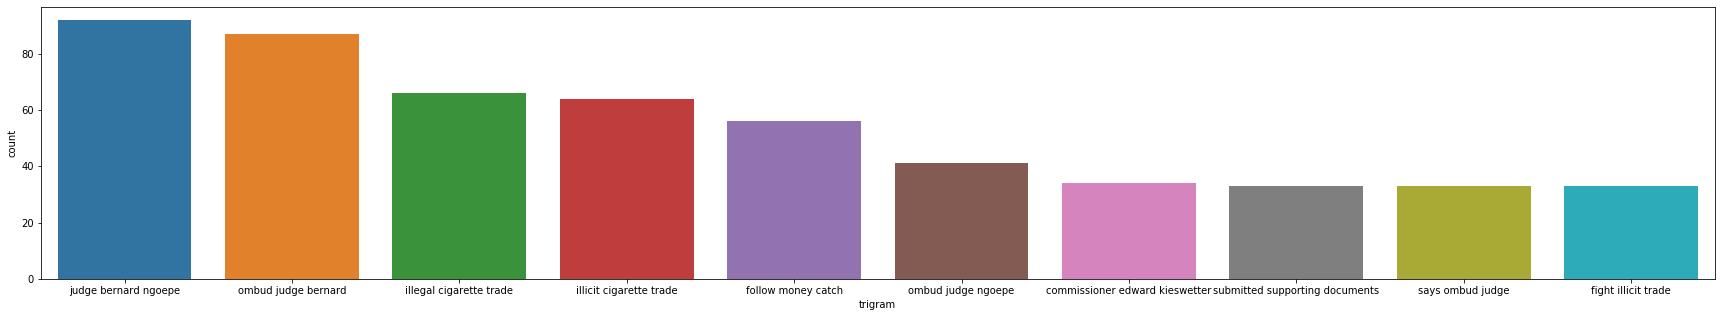
\includegraphics[width=\linewidth]{Tri-gram User Data.png}
		\caption{Tri-Grams outputs for government User}
		\label{fig:Associated Tri-Gram Outputs}
	    \end{subfigure}
	   \vfill
	 \caption{Comparing Bi-Gram vs. Tr-Grams in Phrase Modelling for government user data.}
\end{figure}

Shown by fig 3, with most tweets not containing hashtags the phrase modelling technique was used to assist highlight context of messages by making use of the bi-gram and tri-gram outputs. Mostly, the 2 words which appear together in the top 10 bi-grams coincides with the queries users must have imposed that are service related to the PIT filing season, which indicates that the strategy of customer service oriented government department.  The tri-grams indicate citizens engaging with the department mandate, governance and operations concerns.

Overall, based on the table below few interesting characteristics based on the 7 867 messages.
\begin{itemize}
    \item For every tweet comes with one reply on average. This implies a strategy for social media in a government department that is dedicated to customer service, and responding individually to messages guided by policies.  The outlier shown by a maximum figure of 137 replies relates to a 2021 announcement on,  "We are pleased to announce that a SARS browser solution is now available following issues experienced with the discontinuation of Adobe Flash Player. Thread"
    \item On average every tweet comes retweeted twice.  The outlier of 986 replies is for an announcement on WE ARE HIRING! Some of the capable and highly skilled individuals we need to join us on this exciting journey are: • Chief Data Scientist • Chief Technology &amp; Innovation Officer • Chief Financial Officer • Chief Procurement Officer • Chief Litigation Officer.
    \item On average every tweet comes with 2 likes.
    \item on average tweets are emerging mainly from the 2019 year.
    \item As seen in Fig 5.1 July and August are the most months.
\end{itemize}

\section{User: Citizens}\\

The 7 867 government agency tweets have resulted in 
66 976 tweets data conversation sets with interesting characteristics to monitor engagements for metrics to be examined such as retweets, replies, hashtags, direct messages and overall impact of tweets. 

\begin{itemize}
    \item Time Trends
\end{itemize}

The data description for the 10 year range produced about 66919 entries, with 34 features,  of which 98percent of the data  is for the last 4 years that is 2018 to 2021.  The majority of tweets were observed in the 2021 year, followed by 2020.In 2018 the government agency seem to have strengthened strategy especially on twitter for a business value that is based on relationship building and offering instant support to citizens.\\

\begin{figure}
      \centering
	    \begin{subfigure}{0.1\linewidth}
		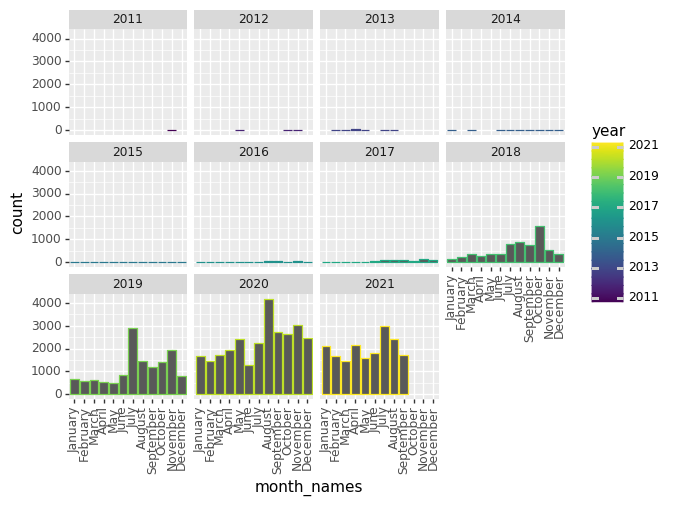
\includegraphics[width=\linewidth]{Overall 10 years of data.png}
		\caption{Overall 10 years}
		\label{fig: 10 year data distribution}
	   \end{subfigure}
	   \begin{subfigure}{0.1\linewidth}
		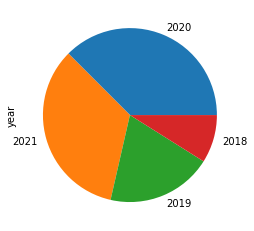
\includegraphics[width=\linewidth]{Annual trends Second Data.png}
		\caption{Four years}
		\label{fig:Four years}
	    \end{subfigure}
	   \vfill
	 \caption{}
\end{figure}

As a result of customer service Twitter strategy the stats below indicate that tweet movement starts early hours in the morning from 5am and gradually slows down early evening at about 7pm, overall users are engaged through out the 24 hour period as shown below.  

Average impressions per tweet by hour tweeted:
----------------------------------------------
20 - 21 : 0.0 =>  525 tweets\\
19 - 20 : 0.0 =>  955 tweets\\
17 - 18 : 0.0 => 2483 tweets\\
15 - 16 : 0.0 => 2965 tweets\\
14 - 15 : 0.0 => 2885 tweets\\
13 - 14 : 0.0 => 3214 tweets\\
12 - 13 : 0.0 => 3766 tweets\\
11 - 12 : 0.0 => 4204 tweets\\
10 - 11 : 0.0 => 4373 tweets\\
 9 - 10 : 0.0 => 4717 tweets\\
 8 -  9 : 0.0 => 4885 tweets\\
 7 -  8 : 0.0 => 5298 tweets\\
 6 -  7 : 0.0 => 5393 tweets\\
 5 -  6 : 0.0 => 5708 tweets\\
 4 -  5 : 0.0 => 4248 tweets\\
 2 -  3 : 0.0 => 1310 tweets\\
21 - 22 : 0.0 =>  291 tweets\\
18 - 19 : 0.0 => 1759 tweets\\
16 - 17 : 0.0 => 2893 tweets\\
 3 -  4 : 0.0 => 2536 tweets\\
 1 -  2 : 0.0 =>  688 tweets\\
 0 -  1 : 0.0 =>  234 tweets\\
23 - 24 : 0.0 =>  211 tweets\\
22 - 23 : 0.0 =>  224 tweets\\

While above it was discussed that on average every tweet posted results in one reply and three likes, some of the tweets may not be responded due to not relating to the specific topic that the customer service oriented government strategy cannot respond to.  However, the point that limited use of hashtags in tweets can result in majority of messages not aligned to a specific topic is valid, with better use of hashtags can effectively connect social media content to a specific topic or event.

\begin{itemize}
    \item Hashtag Analysis
\end{itemize}

More than 80 percentage of the tweets do not have hashtags.  Of those with hashtags used less than 20 percent comes with a possibility of messages not relating to the topic. Overall it would be interesting if the topic modelling results for topics fall within the parameters of the  government agency.

\begin{figure}
    \centering
    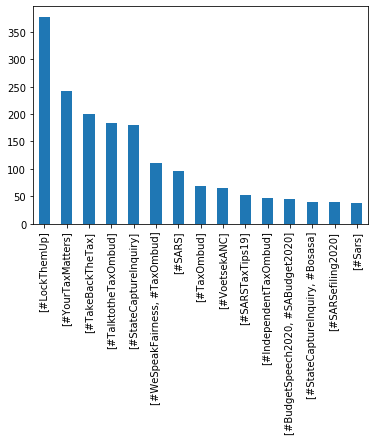
\includegraphics[width=0.1\linewidth]{Hashtags Used Second Data .png}
    \caption{Enter Caption}
    \label{fig:enter-label}
\end{figure}

As seen in Figure 8 below the majority of the communication came though the filing season or campaigns for submissions of returns by individuals taxpayers which occurs mainly between July to September, slowing down in October. This period has the most significant usage of hashtags, such as YourTaxMatters, TaxSeason and with other tax season non-related hashtags such as lockthemup and Statecaptureenquiry.  The tax season hashtags dominating in this period have been following the same trend but higher especially in 2021, which is the year with most tweets for the four main years under study. 

\cite{alsini2021hashtag} It can be beneficial to have correct use of hashtags to contextualize conversations to focus on better engagement(s).  This can lead to greater and quick engagement in users boosting the brand’s social media engagement through likes, shares, comments, and a potential of new followers. Also to bring other topics that may not be important outside the tax season, while eliminating noise and information overload.

\begin{itemize}
    \item Username Analysis
\end{itemize}

It is interesting to note that the dominating usernames other than the "sarstax" are from public figures including tax practitioners - username distribution over the 4-year period shows mainly engagements with civil societies, journalists, tax practitioners, government officials in the public space due to various political reasons.  

\begin{figure}
    \centering
    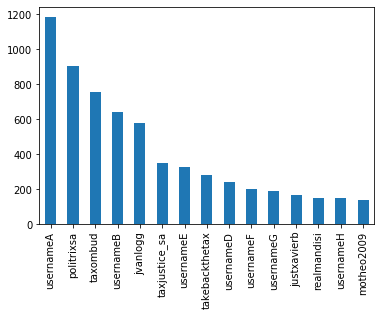
\includegraphics[width=0.1\linewidth]{usenames for second data.png}
    \caption{Enter Caption}
    \label{fig:enter-label}
\end{figure}

\begin{itemize}
    \item Topics 
\end{itemize}

\begin{itemize}
    \item Phrase modelling outputs
\end{itemize}


Looking at the phrase modelling outputs, the tri-grams visualisation output of the top 10 for 3 words which frequently appear together indicates a summary of interesting topics relating to strategy matters.

\begin{figure}
      \centering
	    \begin{subfigure}{0.1\linewidth}
		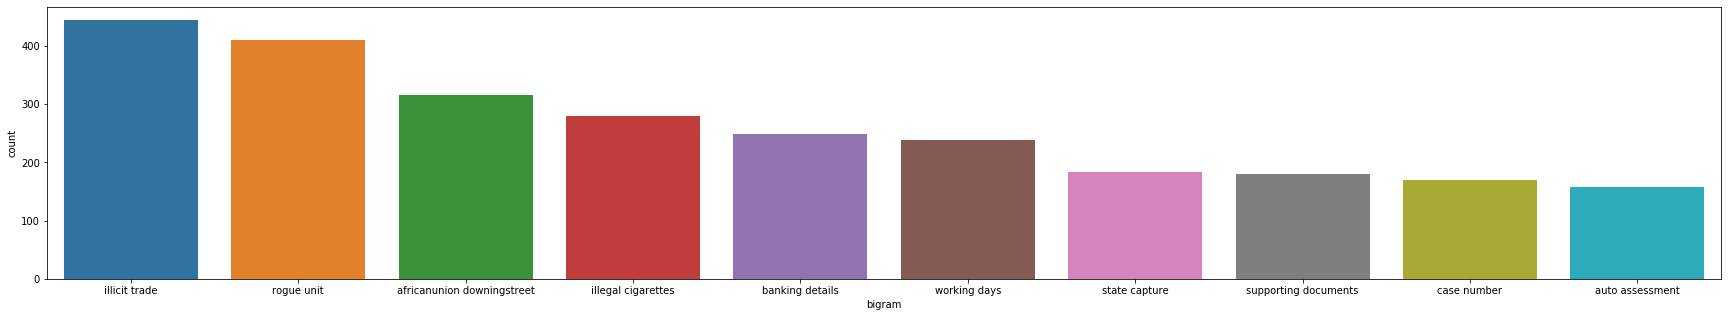
\includegraphics[width=\linewidth]{Bi-grams for second second user data.png}
		\caption{Bi-Grams outputs}
		\label{fig: Associated Bi-Grams Outputs}
	   \end{subfigure}
	   \begin{subfigure}{0.3\linewidth}
		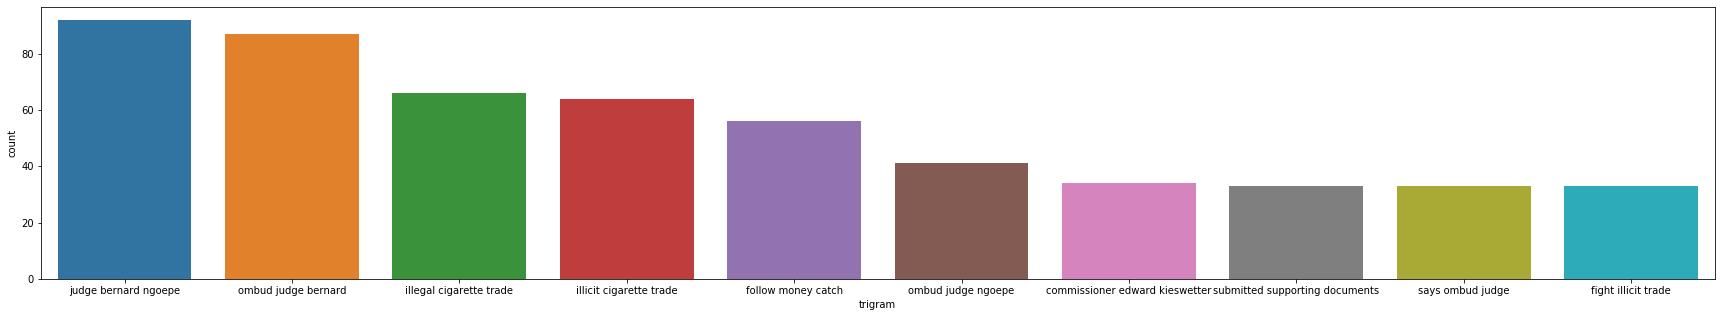
\includegraphics[width=\linewidth]{Tri-gram second second user data.png}
		\caption{Tri-Grams outputs}
		\label{fig:Associated Tri-Gram Outputs}
	    \end{subfigure}
	   \vfill
	 \caption{Comparing Bi-Gram vs. Tr-Grams in Phrase Modelling.}
\end{figure}

Whereas, the bi-grams visualisation for the 2 words which frequently appear together are tax service related on matters taxpayers needed clarity on.

\begin{itemize}
    \item Emerging topics from text analysis
\end{itemize}

The text analysis technique that has been leveraged on to deduce a list of possible topics resulting from overall corpus is the LDA Topic Modelling Technique.  In comparison to other unsupervised topic models algorithms such as the Latent Semantic Indexing (LSI), Hierarchical Dirichlet Process (HDP).  The LDA is more reliable to produce coherent and quality topics when evaluating results with other models as it shows to have better coherence metric values, as shown below.\\

\begin{figure}
      \centering
	    \begin{subfigure}{0.1\linewidth}
		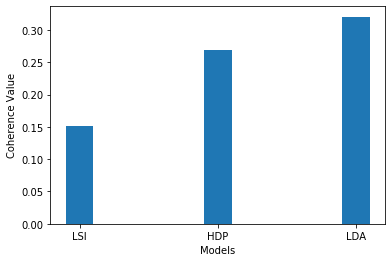
\includegraphics[width=\linewidth]{Evaluate coherence values.png}
		\caption{Coherence values performance }
		\label{fig: Coherence Values}
	   \end{subfigure}
	   \begin{subfigure}{0.1\linewidth}
		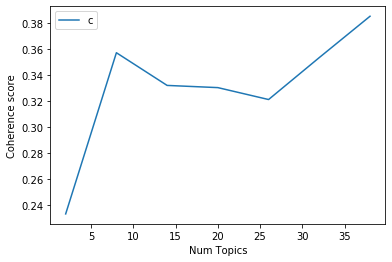
\includegraphics[width=\linewidth]{Number of Topics for the overall data.png}
		\caption{Visual representation of Number of Topics}
		\label{fig:Number of Topics selection}
	    \end{subfigure}
	   \vfill
	 \caption{Comparing topic models coherence values vs  number of topics}
\end{figure}

In order to get the main themes for created topics resulting from the LDA algorithms the process start with the best choice parameters for a finer model by running the CV grid search method to find the best parameters for the LDA.  To initialize  involves feature extraction from the document term matrix of a TF-IDF vector to carry out the topic modelling. The matrix comes with a sparsicity of 0,48 percent following the data processing and removal of stop words, last consideration is the maximum features of 1000.\\
As shown above in fig 9 clearly that the parameter for number of topics =with a value of 10 has a better score for the coherence score of 0.36.\\

Overall results therefore, the base LDA model has the final hyperparameters based on CV Grid search method as follows, the number of topics=10, the learning method for the algorithm updating the assignment of topics to the documents=online, together with the maximum number of iterations to be carried out =10 and the random state = 100.\\
The results are 10 distinct topics despite some topics could share common keywords, it may help to checking for proportion of assigned topics by the model.  In checking the results we can check the proportion of topics that have been assigned to the first document using the lines of code given below.

The table below shows that Topic 10 has the highest proportion

Proportions of topics from the document:\\
\begin{itemize}
    \item Topic  0 :  5.0000000003264145 %\\
\end{itemize}
\begin{itemize}
    \item Topic  1 :  5.000530695799997 %\\
\end{itemize}
\begin{itemize}
    \item Topic  2 :  5.001280907842061 %\\
\end{itemize}
\begin{itemize}
    \item Topic  3 :  5.000000000379809 %\\
\end{itemize}
\begin{itemize}
    \item Topic  4 :  5.0002008679359955 %\\
\end{itemize}
\begin{itemize}
    \item Topic  5 :  5.000000000399167 %\\
\end{itemize}
\begin{itemize}
    \item Topic  6 :  5.000000000336659 %\\
\end{itemize}
\begin{itemize}
    \item Topic  7 :  5.000000000286975 %\\
\end{itemize}
\begin{itemize}
    \item Topic  8 :  5.00028074430452 %\\
\end{itemize}
\begin{itemize}
    \item Topic  9 :  54.9977067823884 %\\
\end{itemize}

For the following 10 topics resulting in the topic modelling LDA technique the results are listed below:

\begin{itemize}
    \item Topic 0: trade report illicit true follow criminals state zuma million reason
\end{itemize}
\begin{itemize}
    \item Topic 1: return working days long audit refund guys returns months year
\end{itemize}
\begin{itemize}
    \item Topic 2: number efiling waiting branch assist submit received today documents response
\end{itemize}
\begin{itemize}
    \item Topic 3: good hope refunds look company file things issue pravin police
\end{itemize}
\begin{itemize}
    \item Topic 4: thank thanks ombud customs exactly believe email address sent compliance
\end{itemize}
\begin{itemize}
    \item Topic 5: unit right commissioner sure start great maybe rogue point minister
\end{itemize}
\begin{itemize}
    \item Topic 6: people problem country like really public question wrong getting white
\end{itemize}
\begin{itemize}
    \item Topic 7: cigarettes paid going paying free taxes read open crime president
\end{itemize}
\begin{itemize}
    \item Topic 8: government illegal corruption business black check court dont evidence years
\end{itemize}
\begin{itemize}
    \item Topic 9: come money stop want details know time need help tell
\end{itemize}

Therefore the topic 10 listed topics from the corpus are listed below as:

When using human judgements to determine the topics are as follows:
\begin{itemize}
    \item Topic 1:  Fight illegal trade activity 
\end{itemize}
\begin{itemize}
    \item Topic 2: long turnaround times post returns submission
\end{itemize}
\begin{itemize}
    \item Topic 3: Minister appointment of commissioner
\end{itemize}
\begin{itemize}
    \item Topic 4:  Appreciatiing tax ombud results
\end{itemize}
\begin{itemize}
    \item Topic 5: Hope for tax refunds appropriateness
\end{itemize}
\begin{itemize}
    \item Topic 6: Minister address rogue unit 
\end{itemize}
\begin{itemize}
    \item Topic 7: Urgent llicit cigarette trade tax crime 
\end{itemize}
\begin{itemize}
    \item Topic 8: Government corruption loosing battle in providing evidence
\end{itemize}
\begin{itemize}
    \item Topic 9:  assistance required case number to query details 
\end{itemize}

Overall the topics discovered through the topic modelling LDA technique realte to the activities for the four years covered. 

\begin{itemize}
    \item Sentiment outputs from text analysis
\end{itemize}

Having explored possible topics from the 4 year engagement discussions, the next is sentiment analysis for overall breakdown engagement of reactions and inputs from users online interaction that can add up emotions from messages with the government department experience over the years covered in the study.  This is to add some quantitative metrics through sentiment analysis in the data exploration analysis.

As messaged add up based on social media use and analysing users comments overtime using a VADER function in python software for a Natural Language Processing (NLP) technique.  
The VADER (Valence Aware Dictionary and sEntiment Reasoner) is a lexicon and rule-based sentiment analysis library of the SentimentIntensityAnalyzer class in Python which returns 4 values, pos, neu, neg and compound.  The compound score is normalised rating of the pos, neu and neg ratings for a single metric value to determine a sentiment. 

The algorithm returns sentiment rating for each tweet for positive, negative and neutral and a compound value to provide a general sentiment of the string.  
While fig 5.14 shows distribution of the normalised compound scores that provides basis for the overall sentiment metric, the actual sentiment scores shows higher neutral sentiments, followed by positive with narrow margin, however the negative sentiment is lowest as shown by Fig 5.15.  At the same time the trend seem to be the same actoss all months of the calendar year depicted in Fig 5.16.\\

\begin{figure}
      \centering
	    \begin{subfigure}{0.1\linewidth}
		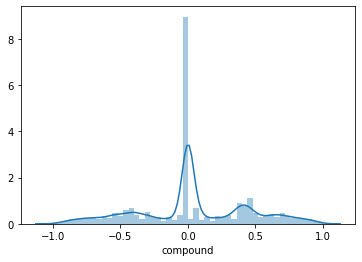
\includegraphics[width=\linewidth]{Sentiment Compound 2.png}
		\caption{Compound results}
		\label{fig:subfig1}
	   \end{subfigure}
	   \begin{subfigure}{0.1\linewidth}
		\includegraphics[width=\linewidth]{Overall Sentiment 2.png}
		\caption{Monthly Sentiments Rating}
		\label{fig:subfig2}
	    \end{subfigure}
	   \vfill
	   \begin{subfigure}{0.1\linewidth}
	   \includegraphics[width=\linewidth]{Overall Sentiments.png}
	   \caption{Overall Sentiment Rating}
	   \label{fig:subfig3}
	   \end{subfigure}
	 \caption{Comparing blue car vs. red car.}
\end{figure}

In all each tweet message has been classified and scored into a sentiment metric of either positive, negative or neutral to get an overview of citizens emotions on their engagements.  It is also possible to observe the sentiments related with the hashtags for the few tweets that have hashtags as shown in Figure and Figure for positive and negative sentiments:\\

\begin{figure}
      \centering
	    \begin{subfigure}{0.1\linewidth}
		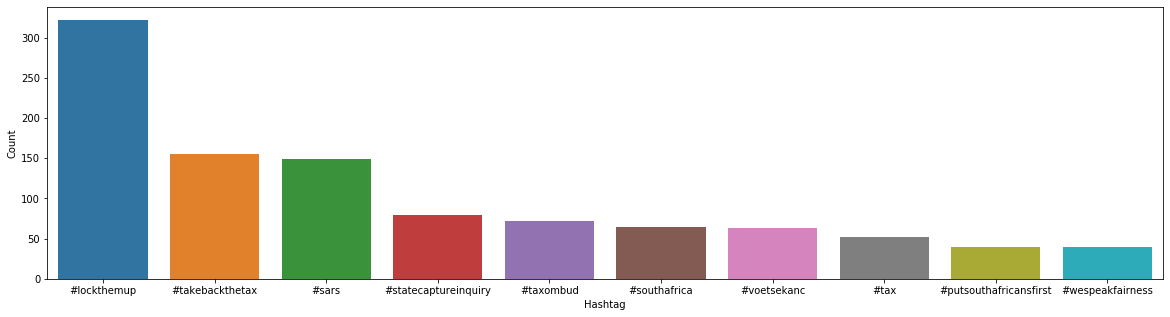
\includegraphics[width=\linewidth]{Sentiments Hashtag Negative.png}
		\caption{Hashtags associated with negative sentiments}
		\label{fig:subfig1}
	   \end{subfigure}
	   \begin{subfigure}{0.1\linewidth}
		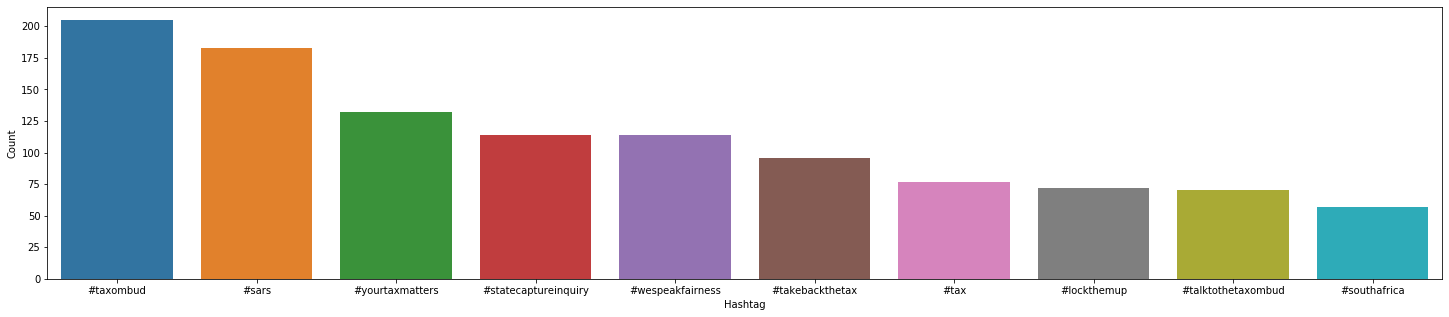
\includegraphics[width=\linewidth]{Hashtag Sentiments Positive.png}
		\caption{Hashtags associated with positive sentiments}
		\label{fig:subfig2}
	    \end{subfigure}
	   \vfill
	 \caption{Comparing blue Negative vs. Positive Sentiment Hashtags.}
\end{figure}

In applying human judgement the possibility of hashtags associated with the sentiments are validated to align\\ 

\subsubsection{Conclusion}

The results of the chapter aim to answer RQ1 abd RQ2 by covering qualitative findings through an exploratory data analysis that has produced results providing insights, understanding including characteristics and behavioural engagements measured between the users, a government and  citizens.\\  Through the ground theory approach for the analysis has revealed results amongst others that users tweets have little usage of hashtags, thus resulting in a hashtag recommendation system to optimise effective use of social media for tweets for the government department under a decade of using twitter.  This chapter is important to give context to the proposed hashtag recommendation solution as a need from the results of user engagements from historical factors.  

\end{document}
\clearpage


\chapter{Literature Review}
\label{chap:lit_review}

This research work brings an intersection of big data analytics outcomes stemming from an e-government communication strategy using internet technologies in a form of social media platforms amongst others for communicating with citizens.  \\
Therefore, literature survey will focus on the two areas, starting to examine e-government communication phenomenon that has evolved overtime in the public sector, followed by social media platforms and big data as an indirect consequence, and concluding by developments in text mining opportunities (machine learning) in the tax environment from big data generated from e-government communication (internet) platforms.  

\subsubsection{e-government}
[E-GOVERNMENT FUNDAMENTALS] E-government can be known by different terms Electronic Governance, Digital Government, Online Government, e-Gov, Electronic Government, "is means to offer services to those within its authority to transact electronically within the government."\\
With majority of citizens using smartphones and access to the internet for applications the digital government innovation is inevitable, [book: ch 22 Thomas Jowazski - From electronic government to policy driven electronic governance evolution of technology use in government], even though "Electronic government is not focused on technology but utilizing technology to improve organization environment within government, on transforming the internal working of government through technology"].\\

[Source: EY Connected Citizen Survey 2020, EYGM Limited 2020.]  In a survey, percentage of citizens who think technology will change, for the better, the way they conduct different tasks - "57percent reported of the entire sample think technology will change, for the better, the way they conduct different tasks.].  In the same study, for the South African sample, 57percent has reported to think that  government and public services are effective in using digital technology to respond to the COVID-19 pandemic?\\
[Making e-gvt work: Adopting the network approach Government Information Quarterly 31 (2014) 327-336], Suggests e-gvt success to use a network explained in 4 critical factors, 1) "Ensuring Availability of resources for success of e-government project", "Ensuring consensus about roles, goals and responsibilities of each other, "Ensuring that electronic process are not replaced/tampered in the long run", "Ensuring smooth functioning of inter-linked processes and facilitating coordination by seamless flow of information", "Ensuring long term commitment of all actors necessary for smooth functioning of the electronic process."\\

[To read Data.gov] and [Government data invisible hand]
The existence of effective interactive participation platforms through social media largely depends on the role played by the public administrator, who may be neutral or a dynamic advocate of citizen participation (Bonsón et al., 2017).\\ 
Public administrators need to mobilise citizens to participate in public issues, collabo-rating in the decision-making process and proposing solutions to the problems of govern- ment (Bonsón et al., 2017; Mergel, 2013b; Zheng and Zheng, 2014), but to achieve this outcome, public administrators must interact with citizens to identify the problems to be addressed so that appropriate solutions may be found and applied (Bonsón et al., 2017; Zafiropoulos et al., 2014).\\
Similarly, Mergel (2013a) observed that attaining a high level of engagement between the society and government means the latter must go beyond the mere publication of content; citizens must be encouraged to comment on government posts to social net- works and to take an active part in this field. In this respect, however, Bonsón et al. (2017) found no relationship between the level of government activity in social media and citizen engagement and suggested that an increase in the number of government posts in channels such as Facebook and Twitter does not necessarily produce higher levels of citizen engagement.\\

Having said that it is also imperative for governments to find innovation to observe and monitor impact of interactive engagements attention with the citizens or users. \\ 

[5]As early as year 2017 the South African government embarked on social media use, after careful consideration of associated risks and governance aspects for legislation providing guidelines to comfortable implement social media technologies, with implementation amongst its departments without a well planned e-government communication strategies. However, [6], this inability of government organizations to go beyond the information broadcasting phase has been highlighted in research (Haro-de-Rosario et al., 2018; Zavattaro, Sementelli, 2014).\\

[Assessing South African Government?s Use of Social Media] This PDF article assesses the use of social media by the South African government for citizen participation. The researchers conducted a qualitative study analyzing the social media pages of South African provinces and municipalities. They found that while all provinces and municipalities have social media accounts, they are mainly used for information broadcasting rather than meaningful engagement and participation. The study highlights the need for a strategy that enhances citizen participation through social media. The researchers categorized the social media use into democratic processes, participation areas, participatory techniques, categories of tools, and technologies. They identified areas such as information provision, service delivery, discourse, consultation, crisis/emergency management, and community building. However, they note that the current use of social media by the South African government is mainly superficial and lacks true public participation. The article concludes by recommending that government organizations post relevant content, actively engage with citizens, and explore the full potential of social media for citizen participation in South Africa.\\
[1] As of January 2021, globally, the active social media users reached 4,29 billion points, and due to increase ownerships of smart devices for the African population of 1,32 billion has 217,5 millions active social media users., despite digital divide for Countries with Developing Economies (CDEs). The digital 2021 report reveals that “ a portfolio approach to social media may help improve efficiency and effectiveness”, an important point for a public administration use of social media.  [3] The e-government initiative is well established and has steadily progressed in a robust two-way communication with citizens.  While effective use of social media efforts in the public sector lacks significant meaningful approach as compared to the private sector, monitoring and evaluation of these efforts is also an important factor for effective and effective strategy to manage efforts also for the public sector. \\
[2]For public administration e-participation amongst others includes social media promoting a two-way communication to transactional between governments and citizens in real time.\\  However, social media effectiveness in government engagement is an area that needs an exploration and investigation for factors such as bureaucracy and overall government ICT policy and strategy can hinder social media purposes and user - government and overall underlying values governing government department ethos.\\
[Chapter 4 Measuring the impact of social media use in the public sector]\\

\begin{table}
    \centering
    \begin{tabular}{cc}
        E-Government & Social Media Use \\
         Static & Bi-directional, interactive\\
         Push information & Pull information\\
         Single author (usually Websmaster) & Multiple factor (providing agency and members of their audiences) \\
         Information or - transaction - focused & Interaction-focused\\
         Large financial investments & Applications created by third parties - free use\\
    \end{tabular}
    \caption{Difference between e-government and social media use in the public sector}
    \label{tab:my_label}
\end{table}

\subsubsection{Social media technologies as e-participation tools in government}

Social media technologies have become essential components to create a two way communication between citizens and government at no costs, as a build up to big data.  

[Gvt as a platfform - Tim O'Reilly], Government 2.0 is the use of technology especially collaborative technologies to better address collective problems facing countries in all levels or spheres of government.  --  This PDF document is an essay written by Tim O'Reilly about the concept of "Government 2.0" and how technology can be used to improve government systems. O'Reilly discusses the power of harnessing the creativity and collaboration of individuals, as seen in successful companies like Google, Amazon, and Wikipedia. He argues that government should adopt a similar approach by using technology to better address collective problems and engage citizens. O'Reilly emphasizes the importance of open standards, simplicity, and designing for participation in creating a successful government platform. He also highlights the value of learning from users and adapting to their needs, as demonstrated by the success of applications like Google Maps. Overall, O'Reilly encourages government to embrace a more innovative and participatory model to improve its services and foster citizen engagement.

[Do E-government Services ‘Really’ Make Life Easier? Analyzing Demographic Indicators of Turkish Citizens’ E-government Perception Using Ordered Response Models, Doi:10.5901/mjss.2015.v6n1p185], while collaborative technologies necessary the question is do they make life easier, so the study demonstrates that effective e-government should promote interaction openly between government and customer.  For continuity, [Digital Government Evolution: from Transformation to Contextualization], Explains the process of expanding digital government in four phases "Digitization", "Transformation", "Engagement" and "Contextualization" thus as an idea for a possible approach. 

"One of key skills required of both technologies and gvt officials is how best to aggregate public opinion or data produced by public actions to reveal new information or patterns" Andy Oram  -- As an opening line even for the abstract.  The importance to have a hashtag recommendation for aggregating granular data into context at the inception level.  

[Big Data and Artificial Intelligence in Policy Making: A Mini- Review Approach] articulates entry and benefits of big data and Artificial Intelligence analytics providing new patterns that opens the closed public sector enhancing communication with customize and on time, rich insights for policy making process.  

[Engaging the Public in Ethical Reasoning About Big Data], Effects of ethical consideration and privacy concerns affect both private (profit/financial interest) and public sector to uphold trust during use of these technologies for order and transparency covering governance.  While  [The complexity of public and private policies for big data], suggests four key elements of the big data policy formulation within the European context, namely, ""Reverberation, nature of expertise, use in backroom deals and changing character and indeed confounding of public and private responsibilities".  

[What does Big Data mean to public affairs research? Understanding the methodological and analytical challenges Big Data for the public sector]The PDF discusses the concept of Big Data in the context of public affairs research. It clarifies the definition of Big Data and highlights its potential as well as limitations in policy making.  The authors emphasize the need for public sector practitioners and researchers to consider methodological, ethical, and analytical challenges when utilizing Big Data. They note that while Big Data offers real-time insights, it may also raise privacy concerns and result in biased predictions due to certain demographics being underrepresented. The authors propose that combining Big Data with administratively collected data and smaller datasets can enhance public programs. However, they stress the importance of understanding the limitations and potential misuse of Big Data.

[Engaging the Public in Ethical Reasoning About Big Data]  -- The PDF document discusses the importance of engaging the public in ethical reasoning about big data. The author emphasizes that the public plays a critical role in privacy and ethical issues related to big data research, and scientists must take public concerns seriously and build trust in specific projects. The chapter explores examples of engaging the public in Wikipedia and contrasts it with "Notice and Consent" forms. The author suggests that scientists should adopt best practices in protecting big data, be transparent about data management practices, make smart choices in deploying digital solutions, and demonstrate a strong commitment to privacy and data security. The document also highlights the ethical concerns in big data and the need for professionals to adapt to new ethical issues related to digital privacy rights. It discusses the implications of the Code (or Architecture), Laws, Markets, and Norms in shaping online activities, and the importance of trust in the efficacy of institutions. The author further explores the public perception of big data, privacy, and digital civil liberties, and the challenges in understanding complex tools for protecting privacy. It emphasizes the need for push technologies and examples of online service providers that have taken steps to improve privacy. The chapter also discusses legal challenges, market-based solutions, and the role of norms in engaging the public. Finally, it presents some practical suggestions for researchers, such as adopting best practices in code and data management, using alternative technologies, and emphasizing the human element in big data research.

[Erschienen in: Public Administration Review ; 76 (2016), 6. - S. 928-937 https://dx.doi.org/10.1111/puar.12625]
Articulates opportunities for real time availability of big data directly from citizens, objectively to enhance immediate operations response by public sector and acting upon citizens needs, relying on capability of data analytics results to open new areas of data insights.  [The Big Data Analysis and Visualization of Mass Messages under “Smart Government Affairs” Based on Text Mining], in this recent study demonstrating public sector use of big data analytics for unstructured of social media sources providing new insights to understand and respond timeously to citizens problems, thus efficiency in government operations to citizens promoted.

[https://doi.org/10.1155/2021/9936217, Research on the Design of Government Affairs Platform in the Context of Big Data.]

The PDF document discusses the design of a government affairs platform in the context of big data. It explores the concepts and theories of big data and analyzes the challenges faced by Chinese government management under the impact of big data. The paper suggests that governments should seize the opportunities that big data brings in terms of management efficiency, administrative capacity, and public services. The design of the government affairs platform is based on service-oriented architecture (SOA) and web services technology. The deep learning algorithm is used to construct a monitoring platform for real-time monitoring of government behavior and analyze the government's intention behavior. The PDF also describes the implementation of the platform using SOAP communication protocol, XML data description, and security measures. Overall, the PDF provides insights into the application of big data in government management and the design of a government affairs platform.

[14] While, social media platforms are instrumental to the production of user generated unstructured data aiding to the big data ecosystem, there are huge  benefits for organisations that have abilities in processing of real-time, short length with appropriate text analytics approach.

[2, 9] Suggest that in order to have a fully utilized government as a strategy for using social media, it is important to anchor this approach with frequent monitoring of effectiveness use of social media.  The social media platform offers dynamic performance that is constantly improving, such as quantity of users, time factors for real-time communication, metadata available due to IoT and increasing content of social media data in real-time.  [14] Introduces a method for effectiveness measurement, a content based predictive analytics recommender which works well with tagged featured data, such as systems with “like” or “dislikes” options.  [15] However, in the absence of tagged features an alternative is to “model a framework designing characteristics to generate user profiles, with aided advantages of semantic entity- and topic-based user modeling strategies”.  

[3] From a view of social networks being instrumental to fullfil a strategic communication purpose for organizations,  through constant monitor of emotional barometer with current, while predictions streamline investments channeling emotions for new users in real-time.  However, lack of research and capabilities of big data infrastructure to store, process, analytics for handling both real-time and batch input datasets for real-time output.

A point of social media analytics gaining  momentum, more effort is also required in developing social media intelligence as a catalyst to provide organizations with context rich frameworks and mechanisms for actionable decision-making [9].   [9, 10] Towards achieving a context rich framework is a social media competitive intelligence, which is a framework that can be used for instance to identify industry trends in comparison to a competitor’s social media performance to benefit specific business operations, in this case this would be for an overall monitoring and evaluation of communication performance in relation to others.  [7] It follows that when social networks are used ethically can be useful to cover various aspects such as, obtain competitive advantage, listening  to users, while participating in conversation with users, shaping relationships from a meaningful content and insights that offers an impactful value appropriation.  

[11] Suggests therefore, Twitter data can enhance required real-time social media response similarly to the application of domain adaption classifiers such as those cover emergency events for disaster response beforehand.   The domain adapted classifiers use machine learning supervised techniques that learns classifiers from both unlabeled targeted data and source label data an  approach uses a Naïve Bayes classifier. 

Overall, text mining techniques can be done through classification, topic modeling, not forsaking sentiment analysis, regression techniques to help understand customers views [17]. 

View from tax authorities

[Comprehensive review of text-mining applications in finance]  -- This PDF article provides a comprehensive review of text-mining applications in finance. The authors discuss the recent literature on text-mining applications in financial forecasting, banking, and corporate finance. They analyze the existing literature on text mining in financial applications, summarize recent studies, and briefly discuss various text-mining methods being applied in the financial domain. The article also highlights the challenges faced in these applications and discusses the future scope of text mining in finance. Key areas covered include sentiment analysis, information extraction, natural language processing, text classification, and deep learning. The authors provide examples of how text mining has been used in financial predictions, such as stock market and forex trends, as well as in banking applications like money laundering prevention. The article concludes with a tabular summary of additional research studies in the field.

Any measure for a return on investment amongst others for social media use are benefits from big data analytics outcomes in government departments including the tax authorities.   Meaning the challenge for discovery of metrics for new data patterns is relevant, and continuously for evaluation of impact for service delivery efforts directly affecting them and cannot be solved elsewhere as public monopolies.   
[4] Since revenue authorities deployment of social media technologies in 2010 with few that had started, however, there is a business sense evident from previous studies that use of social media since it started in 2010 [survey covering 26 revenue authorities to reveal that  measuring effective use of social media] includes metrics such “as the approaches used by revenue bodies to gauge effectiveness were largely confined to numbers of users, visits, views, etc”.  However, some of the suggestions factors to measure:
“Identify influential Twitter followers and number of followers“ for possible presence of visibility to promote two-way communication on relevant “tax-matters”.

“Language and Tweet structure“: Attention to Language and Tweet Structure: Jay Baer points to how social media analytics tools can be useful in evaluating which type of Tweets are successful, the metrics being re-tweets. He suggests that the tools Twitalyzer35 or bit.ly36 data be deployed to see what sort of patterns emerge: Are longer tweets, shorter tweets or those with links most successful? According to Baer on his blog: ―It has (been) found that tweets with links are RT‘d substantially more than tweets without links. 
Tweets asking for help? Know what‘s worked for you in the past, and try to model your future tweeting to mimic it (within reason). 

Repeat your Tweets: Jay Baer states on his blog 37………… ―Yes, it‘s unpopular with the social media purists, but (since) 94percent of tweets are RT‘d within the first hour you need to tap into multiple Twitter audiences throughout the day. I tweet my blog posts 3 times daily, with a different headline each time. This becomes even more important if you have followers in many time zones‖ …… as some revenue bodies do.
\section{The First Section}
\label{sec:second:first_sec}

%%%%%%%%%%%%%%%%%%%%%%%%%%%%%%%%%%%%%%%%%%%%%%%%%
%%%%%%%%%%%%%%%%%%%%%%%%%%%%%%%%%%%%%%%%%%%%%%%%%

\section{The Second Section}
\label{sec:second:second_sec}

%%%%%%%%%%%%%%%%%%%%%%%%%%%%%%%%%%%%%%%%%%%%%%%%%

\subsection{A Subsection}
\label{sec:second:second_sec:one}

%%%%%%%%%%%%%%%%%%%%%%%%%%%%%%%%%%%%%%%%%%%%%%%%%

\subsection{Another Subsection}
\label{sec:second:second_sec:two}

%%%%%%%%%%%%%%%%%%%%%%%%%%%%%%%%%%%%%%%%%%%%%%%%%
%%%%%%%%%%%%%%%%%%%%%%%%%%%%%%%%%%%%%%%%%%%%%%%%%

\section{Summary}
\label{sec:second:summary}

%%%%%%%%%%%%%%%%%%%%%%%%%%%%%%%%%%%%%%%%%%%%%%%%%
%%%%%%%%%%%%%%%%%%%%%%%%%%%%%%%%%%%%%%%%%%%%%%%%%
\clearpage


\bibliographystyle{plain}
\bibliography{dissertation}
\begin{document}

\chapter{Technical Background}
\label{chap:third}

For a comprehensive text analysis outcome in this study, emphasizing the context dimension is crucial for effective understanding, interpretation, and validation of results. The primary focus is on employing a text mining approach to contextualize: 1) topics derived from tax-related Twitter messages, 2) the sentiment analysis corpus, and 3) the application of machine learning prediction techniques for hashtag recommendation within the context of a tax authority. The examination of message data reveals limited use of hashtags initially in categorizing messages on Twitter, a prominent social media platform for a government department.

The rapid increase in messages, comments, and replies has surpassed the capacity for manual sorting and tagging, impeding the provision of operational services required by users. Consequently, natural language processing technology has emerged to identify pressing issues reflected by the public, prompting relevant departments to address them promptly.

\section{Research Methodology}

\subsubsection{Data}

Social media data serves as a key source of intelligence derived from the interactive dynamics between governments and citizens. The study, focusing on social media engagement for a revenue authority, specifically targeted tweets related to a tax government department in South Africa. To ensure a comprehensive representation of two-way interactions, Twitter data was exclusively collected from an account associated with the tax revenue authority. This collection comprised two distinct datasets: one encompassing government posts communicating with citizens, and the other capturing users' responses to these government tweets. The data extraction was centered around tweets containing the keyword "sarstax," a brand-established term, facilitating the identification of both the organization's messages and the corresponding engagements from citizens. Notably, despite the organization's early international inception in 2012, a significant shift in Twitter usage occurred around 2018. This approach ensures that the collected data aligns effectively with the study objectives, providing a robust foundation for analyzing social media interactions in the context of a revenue authority.

\begin{table}
\centering
\begin{tabular}{ |c|c|c|c|}
 \hline
 username & name & place &tweet\\
 language & mentions & urls & photos\\
 replies & count & retweets & count\\
 likes & count & hashtags & cashtags\\
 link & retweet & quote & url\\
 video & thumbnail & near & geo\\
 source & user rtid & user rt & retweet id\\
 reply to & retweet date\\
 \hline
 \end{tabular}
\caption{First table.}
\label{tab:table1}
\end{table}

The 2018 year marks the beginning of social media use in the revenue authority resulting in the annual data collected annually from 2018 up to year 2021. Therefore this chapter will provide a validation of two data sets that have emanated from the government tax authority usage of Twitter social media with citizens. 

\begin{itemize}
    \item Section X emanates from the brand, government tweets
    
    \item Section Y emanates from the users, citizens tweets
\end{itemize}

\subsection{Revenue Authority Tweets} 
These are tweets emanating from the revenue government for the four year period, 2018 - 2021 forming a data set of 7 877 without retweets.  However, according figure [] 13 features in the data set are not populated such as geo, quoteURL, source, near which may be important for segmentation and regional view. 

\begin{figure}[h!]
\centering
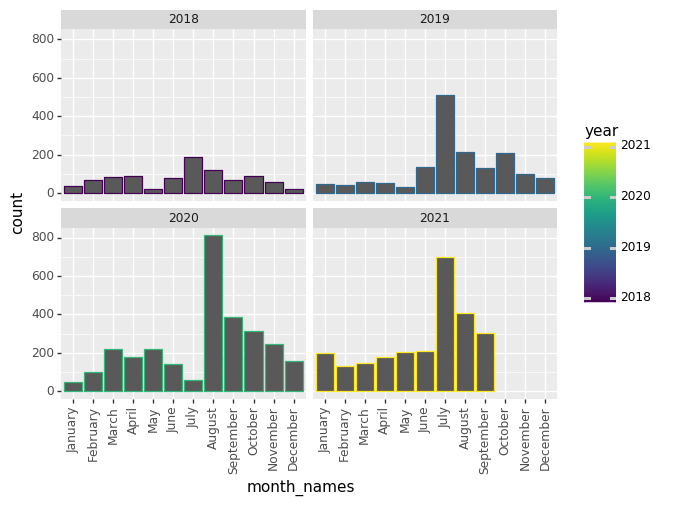
\includegraphics[width=8cm]{postgrad_template 2/Images/Gvt dataset four the four years distribution.png}
\caption{Distribution of GVT Tweets over 4 years.}
\label{fig:figure1}
\end{figure}

Within this dataset, notable aspects of tweet content include 85 percent  lacking hashtags and 26 percent devoid of user mentions. The distribution of tweets per hour reveals a spike during the morning hours, particularly between 4 am and 10 am. Regarding trigrams (3-word sequences), the most frequently repeated phrases include "check profile advice," "send details webmaster," and "send details query."

\subsection{The citizens Tweets} 

The dataset spanning four years comprises 65,919 entries and 34 features, mirroring the number of features in government tweets. Notably, approximately 80 percent of entries lack hashtags. Usernames distribution reveals 11 percent associated with government tweets, followed by 5 percent for civil societies, tax practitioners, and taxpayers each. The most frequently repeated trigrams include "judge bernard ngoepe," "illegal cigarette trade," and "illicit cigarette trade."

\subsection{Tweet Pre-Processing}
The data pre-processing stage entails removing unwanted data features that can make the data noisy for a cleaner data.  In summary the following steps were under taken:

\begin{itemize}
    \item Converting all the tweets into lower case.
\end{itemize}

\begin{itemize}
    \item removal of - duplicated tweets, punctuations, numbers (numeric data); english stop words and domain-related stop words, web links HTML tags(hyperlinks); extra blank spaces; words less than 3 characters;
\end{itemize}

\begin{itemize}
    \item Applied expansion for abbreviations; 
\end{itemize}

\begin{itemize}
    \item "The third step of pre-processing is the normalization of the text under consideration. Normalization is when all the words are brought back to their root level".
\end{itemize}

\begin{itemize}
    \item The second phase involved tokenization, to break larger chunks of data into smaller ones.
\end{itemize}

\subsubsection{Topic Modelling}

In addressing the first part of the RQ1, the age of big data applications and analytics uncovering novel data patterns, this study will employ Latent Dirichlet Allocation (LDA) Topic Model. LDA is an unsupervised machine learning approach designed to extract the meaning from large document corpora, revealing multiple patterns of topics within the text.  According to \cite{blei2011introduction}, Latent Dirichlet Allocation (LDA) is a probabilistic model aimed at uncovering concealed themes within documents, allowing for the inference of hidden topic structures. Alternatively expressed as a soft clustering algorithm, LDA is developed for various applications, including text clustering. In the context of LDA approaches, text clustering implies that each document can encompass multiple scientifically discovered topics, characterized by groups of words that frequently co-occur.
Also \cite{blei2003latent} presents LDA as a generative probabilistic model designed for collections of discrete data. It utilizes a three-level hierarchical Bayesian model to formulate topics, making it applicable to the analysis of social media data. This model illustrates the process by which a specific text corpus might have been generated from certain topics. An illustrative example is [How to identify topics in psychology using topic modeling], showcasing the application of Topic Modeling based on LDA to understand trending topics in psychology research within a large collection of documents.
\cite{mabey2018pyldavis}The exploration and presentation of discovered topics through topic models, allowing for a thorough examination of the relationships between topics and terms in an LDA model, can be facilitated by "PLDAvis," a tool accessible in Python. This tool helps address questions such as: 1) "What is the meaning of each topic?", 2) "How prevalent is each topic?", and 3) "How do the topics relate to each other?"

\subsubsection{Sentiment Analysis}

This subsection also addresses Research Question 2, which explores the evolution of computer-based sentiment analysis. Initially, sentiment analysis was limited to subjective texts available on the web and focused on online product reviews. However, post-2014, the focus shifted to social media texts, particularly from Twitter and Facebook. The significance of incorporating LDA topic modeling alongside qualitative coding for clustering is emphasized.

\cite{liu2010sentiment} describes sentiment analysis involving a series of methods, techniques, and tools for detecting and extracting subjective information, such as opinions and attitudes from language.

The outcomes of sentiment analysis/prediction encompass the labeling of each tweet/retweet based on sentiment polarity. This process enables the calculation/coding of sentiment distribution over time, providing insights into the evolving trends in citizens' behavior in response to government tweets. The final result is a visual representation of monthly sentiment trends, which assists in recognizing significant events/announcements. This strategy is enhanced by insights drawn from Topics/Wordclouds derived through topic modeling. The rationale for integrating both methods is consolidated within the Exploratory Data Analysis (EDA), while the primary focus of the methodology remains on hashtag recommendation.

\subsubsection{Hashtag Recommendation}

\cite{alsini2021hashtag} provides a review of methods for hashtag recommendation on social media platforms, specifically Twitter and Sina Weibo. The authors conduct a systematic literature review to gather research papers on this topic published between 2010 and 2020, discovering that most of the research focuses on the textual content of tweets and that collaborative filtering methods are rarely used in hashtag recommendation. Based on their findings, they propose a taxonomy of hashtag recommendation methods, including text-based methods, hybrid user-based methods, and hybrid miscellaneous methods. They also discuss the challenges and future research directions in this field.

\cite{zhao2016personalized} The paper presents a personalized hashtag recommendation approach using a Latent Dirichlet Allocation (LDA)-based topic model in a microblog environment. The approach combines user profile-based collaborative filtering and LDA-based collaborative filtering to find relevant hashtags for users. The proposed LDA-based model, called Hashtag-LDA, jointly models the relationships between users, hashtags, and words in microblogs. The experimental results on a real Twitter dataset show that the proposed recommendation approach outperforms other related methods and that Hashtag-LDA is effective in finding relevant hashtags.

\cite{godin2013using} this paper introduces an unsupervised and content-based hashtag recommendation method for tweets. The approach utilizes Latent Dirichlet Allocation (LDA) to model the underlying topic assignment of language-classified tweets. The key advantage lies in using a topic distribution for recommending general hashtags. The paper covers related work, details the process of creating a tweet dataset, and outlines the binary classification algorithm used to classify tweets as English or non-English language. The conclusion includes evaluation results and outlines future work. The content-based method employs Latent Dirichlet Allocation (LDA), a hidden generative topic model, enhancing effective categorization and search of tweets while mitigating sparse and noisy tweet content.

\cite{mehrotra2013improving} at the same time addresses challenges in applying topic models, particularly Latent Dirichlet Allocation (LDA), to Twitter content due to the concise and unstructured nature of tweets. The paper investigates various pooling schemes, emphasizing tweet pooling by hashtags, to enhance the quality of topics derived from Twitter data. Through empirical evidence, the authors show that hashtag-based pooling significantly improves topic coherence compared to other schemes and the baseline LDA model. Additionally, the automatic labeling of hashtags further enhances topic quality. The paper offers valuable insights and methods for improving LDA topic models when applied to Twitter content.

This PDF discusses the development of an interactive hashtag recommendation system for social media platforms like Twitter. The system aims to help users enhance their tweets by suggesting relevant hashtags. The system consists of two phases: divergence and convergence. In the divergence phase, the system provides users with related topics based on their input tweet, allowing them to explore novel hashtags. In the convergence phase, the system recommends more accurate hashtags based on the selected topic. The system utilizes natural language processing, topic modeling, and recommendation algorithms to achieve accurate and efficient hashtag recommendations. The system's effectiveness and usability were evaluated through user experiments, with positive results indicating that the interactive hashtag recommendation system provides accurate and helpful hashtags for users.

\cite{alsini2021hashtag} brings a discussion n the development of an interactive hashtag recommendation system for social media platforms like Twitter. The system aims to help users enhance their tweets by suggesting relevant hashtags. The system consists of two phases: divergence and convergence. In the divergence phase, the system provides users with related topics based on their input tweet, allowing them to explore novel hashtags. In the convergence phase, the system recommends more accurate hashtags based on the selected topic. The system utilizes natural language processing, topic modeling, and recommendation algorithms to achieve accurate and efficient hashtag recommendations. The system's effectiveness and usability were evaluated through user experiments, with positive results indicating that the interactive hashtag recommendation system provides accurate and helpful hashtags for users.

\cite{altinel2018semantic} discusses the topic of semantic text classification, which is the task of organizing documents into pre-determined classes using machine learning algorithms. It highlights the importance of capturing the semantics of words and the semantic connections between words, documents, and classes in order to achieve better classification performance. The PDF reviews knowledge-based approaches, such as the use of WordNet, Wiktionary, and Wikipedia as domain knowledge sources, and discusses their advantages over traditional text classification methods. It also explores corpus-based approaches that utilize statistical analysis to discover hidden connections between words in training documents. Additionally, the PDF covers deep learning-based approaches, methods that enhance word/character sequences, and linguistic enriched approaches for semantic text classification. The performance comparison of these approaches is discussed, along with their experimental results and advantages / disadvantages. Overall, the PDF provides a comprehensive overview of semantic text classification and the various approaches used in the field.

Inspired by Community question answering websites that have used both questions text or tags (keywords related to the asked question) topic modelling can summarize and describe content of the question, in this case the extension to understand the context of the tweet for themes and topics of discussion.

\cite{prabha2023question} conducted a study to support that using a text for topic modelling is producing better performance as opposed to using tags when evaluated model using tw metrics namely coherence and perplexity.  In using the users data  (tweets/text), one can determine the hidden information about the user and trending topics across domains.  Hashtags and tags provide context regarding context and semantics.

1. Data Preprocessing:
   - Tokenize the tweets: Split each tweet into individual words or tokens.
   - Remove stop words: Remove common words like "the," "is," "and," etc., as they don't contribute much to the hashtag recommendation process.
   - Stemming/Lemmatization: Reduce words to their base or root form (e.g., "running" becomes "run").
   - Vectorization: Convert the preprocessed tweets into numerical feature vectors using techniques such as TF-IDF.

2. Supervised Model Training:
   - Random Forest Classifier (RFC): Train an RFC model using the preprocessed tweet vectors and their corresponding hashtags as labels.
   - Support Vector Classifier (SVC): Train an SVC model using the same preprocessed tweet vectors and hashtag labels.

3. Unsupervised Topic Model Training:
   - Latent Dirichlet Allocation (LDA): Apply LDA to the preprocessed tweet vectors to discover latent topics within the tweet corpus.

4. Hashtag Recommendation:
   - Given a new tweet, pre-process it and convert it into a feature vector.
   - Use the trained RFC and SVC models to predict the most relevant hashtags for the tweet.
   - Utilize the LDA model to identify the latent topics in the tweet and suggest hashtags related to those topics.
   - The model only Utilized the 7887 tweet messages with identifiable hashtags
This has resulted to recommendation of topics of tweets to organise with an appropriate hashtag for improved user experience that can lead to an efficient two-way communication resulting in organization better services through continuous evidence-based decision making efforts.

\subsubsection{Model Evaluation}

[EVALUATION technique METRIC FOR HASHTAG RECOMMENDATION] The paper examines the assessment of metrics for hashtag recommendation systems, which automatically suggest hashtags to users while composing a tweet. The authors contend that widely used metrics such as hit rate, precision, recall, and F1-score may be insufficient for evaluating hashtag recommendation systems, particularly when the number of ground truth hashtags in tweets varies greatly. They introduce a novel metric termed "hit ratio" to address this issue, considering the varying number of hashtags in the recommended and ground truth sets. The hit ratio is computed as the ratio of matching hashtags over the minimum value between the number of recommended hashtags and the number of ground truth hashtags. The authors compare the hit ratio with traditional evaluation metrics, illustrating its utility through hypothetical scenarios and real-world applications. They assert that the hit ratio offers a more meaningful metric than traditional measures for the evaluation of hashtag recommendation systems.

Some of the evaluation metrics which can be used both for supervised and unsupervised techniques:

\begin{itemize}
    \item Jaccard Score: Calculates the Jaccard similarity score between the predicted hashtags and the actual hashtags for a set of test tweets. Jaccard score measures the similarity between two sets of hashtags.\\
\end{itemize}
\begin{itemize}
    \item Dummy Classifier: Build a dummy classifier to predict whether a tweet is  using the pre-processed tweet vectors for an appropriate hashtag.
\end{itemize}

\begin{itemize}
    \item to iterate and fine-tune the models and evaluation metrics based on the specific characteristics of your tweet dataset and the desired performance.
\end{itemize}
\begin{itemize}
    \item In order to evaluate the text classification supervised models in Topic Modelling unsupervised method to determine their effectiveness in analyzing short text data.   The topic modelling evaluation method is based on "the understandability of extracted topics (topic quality) besides the topic performance and accuracy by applying common standard metrics that apply to the TM domain such as recall, precision, F-score, and topic coherence".
\end{itemize}


\subsubsection{Conclusion}

In conclusion the research methodology has emphasized the importance of understanding the context and domain-specific requirements when selecting and evaluating the algorithms for hashtag recommendation. By considering the unique characteristics of Twitter or the government department's data collection efforts, the researcher has streamlined the methodology to suit the specific needs and challenges of the government environment.
In summary, the research methodology presented in this chapter provides a robust framework for text mining and production techniques aimed at recommending hashtag tags. By combining supervised and unsupervised algorithms, we have demonstrated the potential for enhancing the accuracy and efficiency of hashtag recommendation processes for Twitter or a government department involved in data collection and analysis. This methodology serves as a foundation for the subsequent stages of our research, enabling us to delve deeper into the implementation and evaluation of these techniques and ultimately contribute to the advancements in the field of text mining and recommendation systems."

\bibliographystyle{plain}
\bibliography{dissertation}

\end{document}







\clearpage


\chapter{Thew Exploratory Data Analysis}
\label{chap:chapter4}

\section{Introduction}

The use of social media technology tools in government can be effective to  achieve digital footprint to streamline the delivery of services and user engagement.  The research study initiates by exploratory analysis of Twitter data set generated by users for a period from 2016 to 2021, indirectly generating big data and through analytics capabilities to uncover hidden patterns from historical data to aid future decision making.   The outcomes of the chapter is mainly comprised of firstly descriptive aspects an analytic process to uncover twitter behavioural characteristics to address first RQ1. This is done by measuring engagement between government and public users on twitter, by exploring features and trends of behaviour over time.  Secondly to answer the RQ2, with further reviewing overall trending topics for the four year summarised to provide insights of past conversations and determined sentiments ratings as results from text mining of a tax government department in analytic outcomes.  Overall outcome of the chapter will guide necessary machine learning use (RQ3) for future solution based on hindsight from data insight in understanding engagement, behaviour characteristics for participation for effective use of Twitter by the government agency to make a difference.\\

\subsection{User Government Agency}

With the government agency as Twitter user with an interaction with citizens with rigour from 2018 to 2021 has accumulated in 7 896 messages indicating a strategy of customer service agency, a transactional tactic based on a dedicated social media team that can offer individualised responses as shown by the analysis.

The exploration of social media data through analytics is an important step to understand engagement behaviour between users as contributors to the data.  This data has been acted upon for exploring data characteristics aspects and features such as likes, retweeted messages, replies messages while providing understanding at a glance engagement aspects up to the topics and overall sentiments.  Therefore, the framework that has guided the research methods for the study data analysis and experiment needed is the ground theory approach guided by the exploratory analysis results.  This approach has discovered that users tweets have little usage of hashtags, thus resulting in a hashtag recommendation system to optimize effective use of social media for tweets for the government department under a decade of using twitter.\\
By looking at the average impressions of the number of times a tweet has been seen by users on the social media platform," to track the reach and engagements of tweets to determine the impact of their content on Twitter.\\
The user activity in terms of time is at the highest early hours of the morning, from 05h00 until midday, while seems to stop at about 9pm.\\
The user data does not contain any retweets.  Hence any other duplicates were removed for an amount of 7 867 tweets originating from the government agency.\\
Overall, about 26 percent (2 059)of tweets have not been replied to, meaning the more than 70 percent of tweets have been replied to by the government agency in relation to its social media policy.  This implies a customer service Twitter Strategy for a government department with dedicated staff responding to tweets with assistance of knowledge experts inside the organisation.\\

\begin{itemize}
    \item User participation (Time and Months)
\end{itemize}

Average impressions per tweet by hour tweeted:
----------------------------------------------
12 - 13 : 0.0 = 487 tweets\\
11 - 12 : 0.0 = 675 tweets\\
 8 - 9  : 0.0 = 707 tweets\\
 7 - 8  : 0.0 = 826 tweets\\
 6 - 7  : 0.0 = 957 tweets\\
 5 - 6  : 0.0 = 1361 tweets\\
14 - 15 : 0.0 = 126 tweets\\
10 - 11 : 0.0 = 730 tweets\\
 4 - 5  : 0.0 = 681 tweets\\
13 - 14 : 0.0 = 252 tweets\\
 9 - 10 : 0.0 = 793 tweets\\
 3 - 4  : 0.0 = 111 tweets\\
15 - 16 : 0.0 = 53 tweets\\
16 - 17 : 0.0 = 23 tweets\\
18 - 19 : 0.0 = 4  tweets\\
20 - 21 : 0.0 = 3  tweets\\
 2 - 3  : 0.0 = 49 tweets\\
 1 - 2  : 0.0 = 20 tweets\\
17 - 18 : 0.0 = 18 tweets\\
19 - 20 : 0.0 = 1  tweets\\

Time trends show an urgency dedicated to customer service department strategy with engagement of more than 12 hours in a day.   The first year for the user (department) Twitter full implementation of social media strategy in 2016 as evidently shown in fig 1, since then  there has been a sturdy increase in its usage, in all the 4 yeas shown the most busiest months are mainly July, August, September and October.  These are months associated with individual filing of returns for the tax Season which starts in July.\\

\begin{figure}
      \centering
	    \begin{subfigure}{0.3\linewidth}
		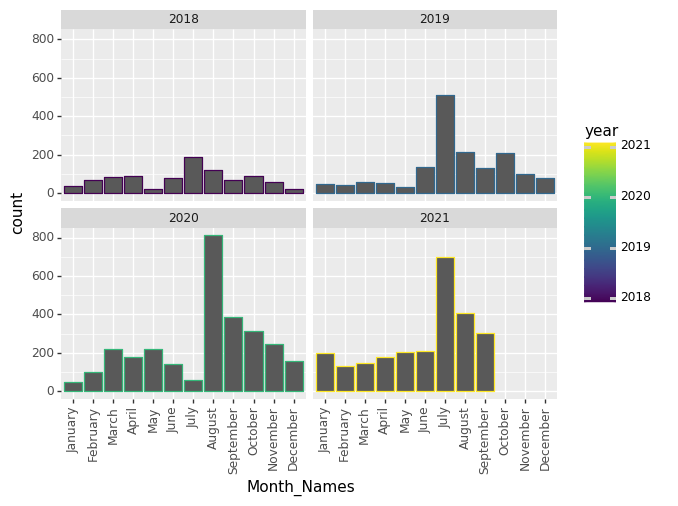
\includegraphics[width=\linewidth]{Users Month Names.png}
		\caption{Monthly engagements}
		\label{fig: Monthly Breakdown for engagement}
	   \end{subfigure}
	   \begin{subfigure}{0.3\linewidth}
		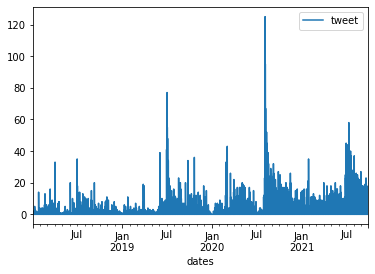
\includegraphics[width=\linewidth]{User 1 Minute Count.png}
		\caption{Time trends outputs}
		\label{fig:Breakdown of time trends by minute}
	    \end{subfigure}
	   \vfill
	 \caption{Time Comparison Monthly vs. Minutes in user engagement.}
\end{figure}

\begin{itemize}
    \item Hashtag Analysis
\end{itemize}

Another aspect to consider is hashtag use, in total for the 7 867 unique records of tweets, only 729 tweets have some representation of hashtags, meaning that 91 percent of tweets do not have any hashtags.  As a result of peaks in Twitter during the tax season for submission of returns by individuals, despite less than 15 percent of tweets use hashtags. The most popular used hashtags are in relation to the context of the filing season, YourTaxMatters(219), SARSTaxTips19(48), TaxSeason2018 (26), SARSRevenueAnnouncement(24), BRICS10Customs(22).\\

\begin{figure}
    \centering
    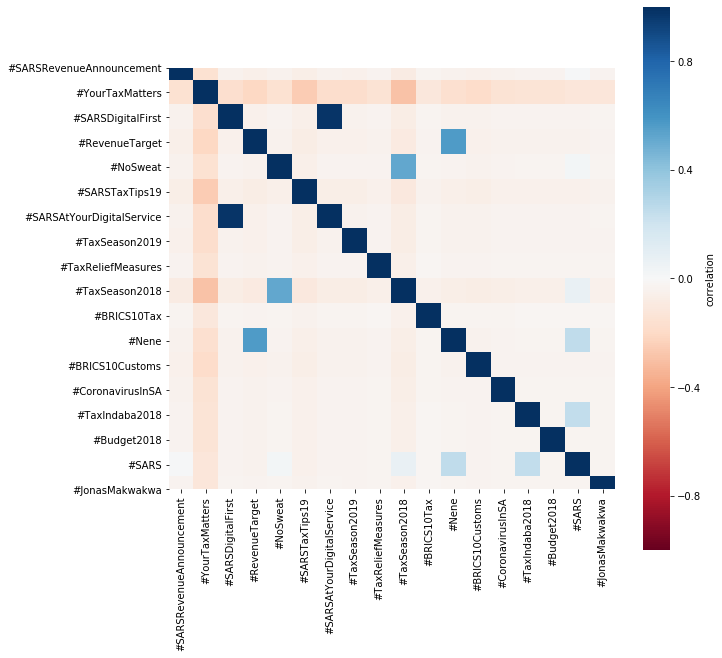
\includegraphics[width=0.5\linewidth]{User Hashtag Correlation.png}
    \caption{Hashtag correlation output}
    \label{fig:Hashtag correlation for government user}
\end{figure}

The correlation matrix shows the following relationship between the most used hashtags
\begin{itemize}
    \item SARSTaxTips19 has a strong positive relationship with YourTaxMatters.  
    \item TaxSeason2018 has a negative relationship with YourTaxMatters.  
    \item TaxSeason2018 has a strong positive relationship with Nosweat
    \item  Nene has a positive relationship with RevenueTarget
    \item  Nene has a positive relationship with SARS 
\end{itemize}

This could mean sending of tax tips in 2019 tax year were helpful for the tax season activities.  The 2018 tax season was not so instrumental.  However, at the same time for the 2018 with a strong support of no sweat campaigns.  Nene had a favourable revenue announcement for tax collection and with SARS in general.

\begin{figure}
      \centering
	    \begin{subfigure}{0.6\linewidth}
		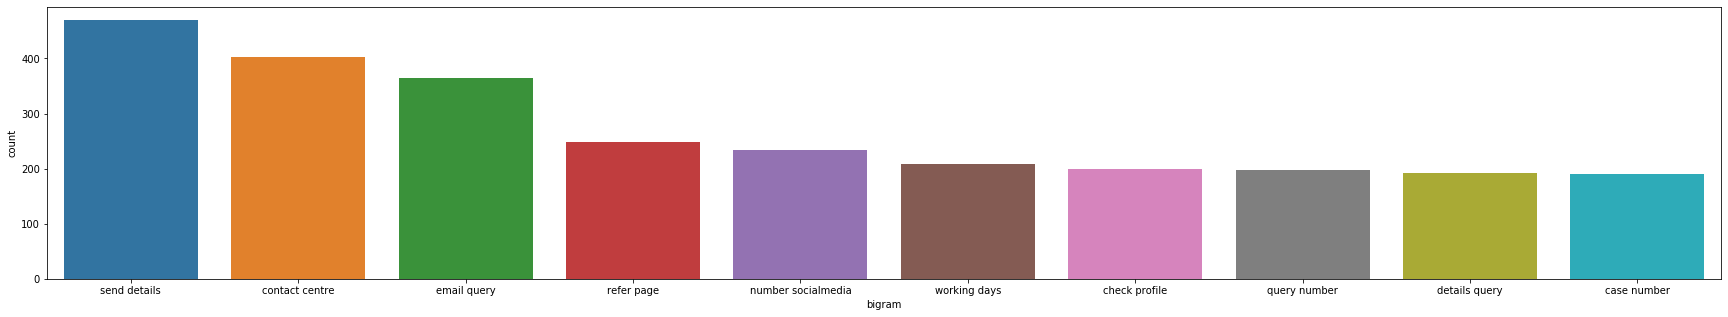
\includegraphics[width=\linewidth]{Bigrams User Data.png}
		\caption{Bi-Grams outputs for government User}
		\label{fig: Associated Bi-Grams Outputs}
	   \end{subfigure}
	   \begin{subfigure}{0.6\linewidth}
		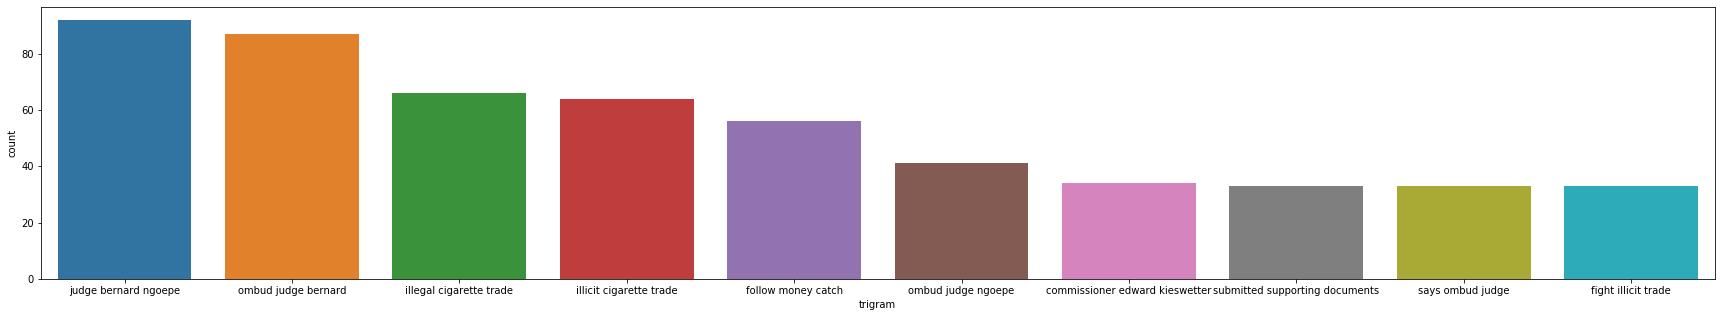
\includegraphics[width=\linewidth]{Tri-gram User Data.png}
		\caption{Tri-Grams outputs for government User}
		\label{fig:Associated Tri-Gram Outputs}
	    \end{subfigure}
	   \vfill
	 \caption{Comparing Bi-Gram vs. Tr-Grams in Phrase Modelling for government user data.}
\end{figure}

Shown by fig 3, with most tweets not containing hashtags the phrase modelling technique was used to assist highlight context of messages by making use of the bi-gram and tri-gram outputs. Mostly, the 2 words which appear together in the top 10 bi-grams coincides with the queries users must have imposed that are service related to the PIT filing season, which indicates that the strategy of customer service oriented government department.  The tri-grams indicate citizens engaging with the department mandate, governance and operations concerns.

Overall, based on the table below few interesting characteristics based on the 7 867 messages.
\begin{itemize}
    \item For every tweet comes with one reply on average. This implies a strategy for social media in a government department that is dedicated to customer service, and responding individually to messages guided by policies.  The outlier shown by a maximum figure of 137 replies relates to a 2021 announcement on,  "We are pleased to announce that a SARS browser solution is now available following issues experienced with the discontinuation of Adobe Flash Player. Thread"
    \item On average every tweet comes retweeted twice.  The outlier of 986 replies is for an announcement on WE ARE HIRING! Some of the capable and highly skilled individuals we need to join us on this exciting journey are: • Chief Data Scientist • Chief Technology &amp; Innovation Officer • Chief Financial Officer • Chief Procurement Officer • Chief Litigation Officer.
    \item On average every tweet comes with 2 likes.
    \item on average tweets are emerging mainly from the 2019 year.
    \item As seen in Fig 5.1 July and August are the most months.
\end{itemize}

\section{Conversations with engaged citizens}\\

The 7 867 government agency tweets have resulted in 
66 976 tweets data conversation sets with interesting characteristics to monitor engagements for metrics to be examined such as retweets, replies, hashtags, direct messages and overall impact of tweets. 

\begin{itemize}
    \item Time Trends
\end{itemize}

The data description for the 10 year range produced about 66919 entries, with 34 features,  of which 98percent of the data  is for the last 4 years that is 2018 to 2021.  The majority of tweets were observed in the 2021 year, followed by 2020.In 2018 the government agency seem to have strengthened strategy especially on twitter for a business value that is based on relationship building and offering instant support to citizens.\\

\begin{figure}
      \centering
	    \begin{subfigure}{0.3\linewidth}
		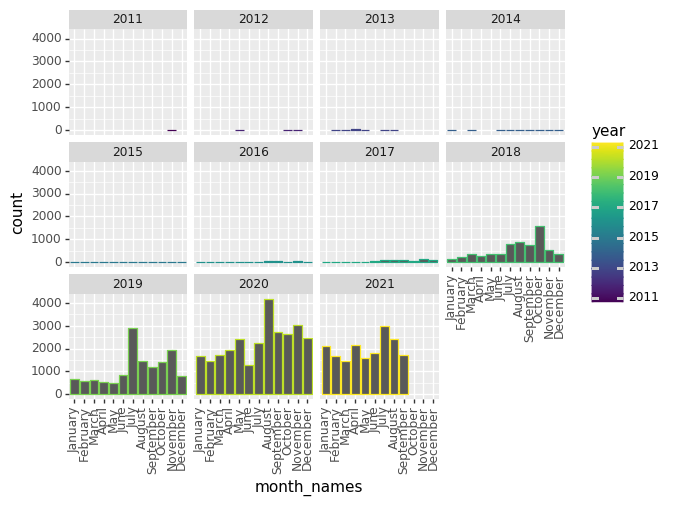
\includegraphics[width=\linewidth]{Overall 10 years of data.png}
		\caption{Overall 10 years}
		\label{fig: 10 year data distribution}
	   \end{subfigure}
	   \begin{subfigure}{0.3\linewidth}
		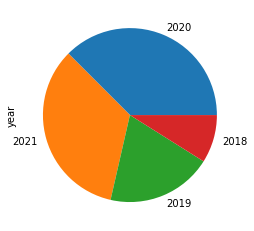
\includegraphics[width=\linewidth]{Annual trends Second Data.png}
		\caption{Four years}
		\label{fig:Four years}
	    \end{subfigure}
	   \vfill
	 \caption{}
\end{figure}

As a result of customer service Twitter strategy the stats below indicate that tweet movement starts early hours in the morning from 5am and gradually slows down early evening at about 7pm, overall users are engaged through out the 24 hour period as shown below.  

Average impressions per tweet by hour tweeted:
----------------------------------------------
20 - 21 : 0.0 =>  525 tweets\\
19 - 20 : 0.0 =>  955 tweets\\
17 - 18 : 0.0 => 2483 tweets\\
15 - 16 : 0.0 => 2965 tweets\\
14 - 15 : 0.0 => 2885 tweets\\
13 - 14 : 0.0 => 3214 tweets\\
12 - 13 : 0.0 => 3766 tweets\\
11 - 12 : 0.0 => 4204 tweets\\
10 - 11 : 0.0 => 4373 tweets\\
 9 - 10 : 0.0 => 4717 tweets\\
 8 -  9 : 0.0 => 4885 tweets\\
 7 -  8 : 0.0 => 5298 tweets\\
 6 -  7 : 0.0 => 5393 tweets\\
 5 -  6 : 0.0 => 5708 tweets\\
 4 -  5 : 0.0 => 4248 tweets\\
 2 -  3 : 0.0 => 1310 tweets\\
21 - 22 : 0.0 =>  291 tweets\\
18 - 19 : 0.0 => 1759 tweets\\
16 - 17 : 0.0 => 2893 tweets\\
 3 -  4 : 0.0 => 2536 tweets\\
 1 -  2 : 0.0 =>  688 tweets\\
 0 -  1 : 0.0 =>  234 tweets\\
23 - 24 : 0.0 =>  211 tweets\\
22 - 23 : 0.0 =>  224 tweets\\

While above it was discussed that on average every tweet posted results in one reply and three likes, some of the tweets may not be responded due to not relating to the specific topic that the customer service oriented government strategy cannot respond to.  However, the point that limited use of hashtags in tweets can result in majority of messages not aligned to a specific topic is valid, with better use of hashtags can effectively connect social media content to a specific topic or event.

\begin{itemize}
    \item Hashtag Analysis
\end{itemize}

More than 80 percentage of the tweets do not have hashtags.  Of those with hashtags used less than 20 percent comes with a possibility of messages not relating to the topic. Overall it would be interesting if the topic modelling results for topics fall within the parameters of the  government agency.

\begin{figure}
    \centering
    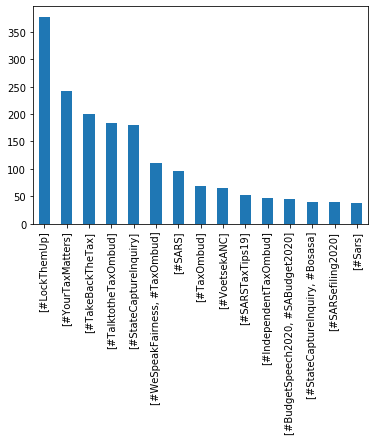
\includegraphics[width=0.5\linewidth]{Hashtags Used Second Data .png}
    \caption{Enter Caption}
    \label{fig:enter-label}
\end{figure}

As seen in Figure 8 below the majority of the communication came though the filing season or campaigns for submissions of returns by individuals taxpayers which occurs mainly between July to September, slowing down in October. This period has the most significant usage of hashtags, such as YourTaxMatters, TaxSeason and with other tax season non-related hashtags such as lockthemup and Statecaptureenquiry.  The tax season hashtags dominating in this period have been following the same trend but higher especially in 2021, which is the year with most tweets for the four main years under study. 

\cite{alsini2021hashtag} It can be beneficial to have correct use of hashtags to contextualize conversations to focus on better engagement(s).  This can lead to greater and quick engagement in users boosting the brand’s social media engagement through likes, shares, comments, and a potential of new followers. Also to bring other topics that may not be important outside the tax season, while eliminating noise and information overload.

\begin{itemize}
    \item Username Analysis
\end{itemize}

It is interesting to note that the dominating usernames other than the "sarstax" are from public figures including tax practitioners - username distribution over the 4-year period shows mainly engagements with civil societies, journalists, tax practitioners, government officials in the public space due to various political reasons.  

\begin{figure}
    \centering
    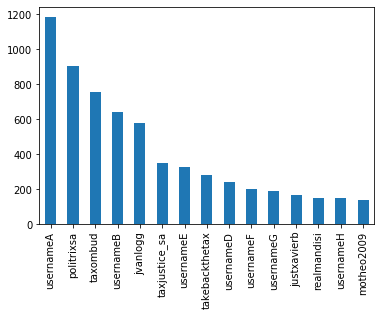
\includegraphics[width=0.5\linewidth]{usenames for second data.png}
    \caption{Enter Caption}
    \label{fig:enter-label}
\end{figure}

\begin{itemize}
    \item Topics 
\end{itemize}

\begin{itemize}
    \item Phrase modelling outputs
\end{itemize}


Looking at the phrase modelling outputs, the tri-grams visualisation output of the top 10 for 3 words which frequently appear together indicates a summary of interesting topics relating to strategy matters.

\begin{figure}
      \centering
	    \begin{subfigure}{0.25\linewidth}
		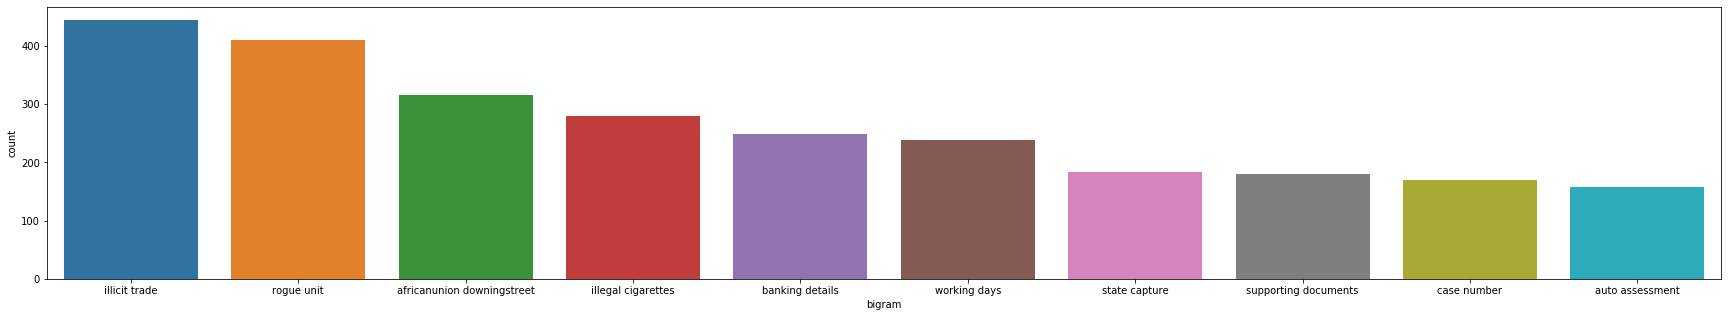
\includegraphics[width=\linewidth]{Bi-grams for second second user data.png}
		\caption{Bi-Grams outputs}
		\label{fig: Associated Bi-Grams Outputs}
	   \end{subfigure}
	   \begin{subfigure}{0.25\linewidth}
		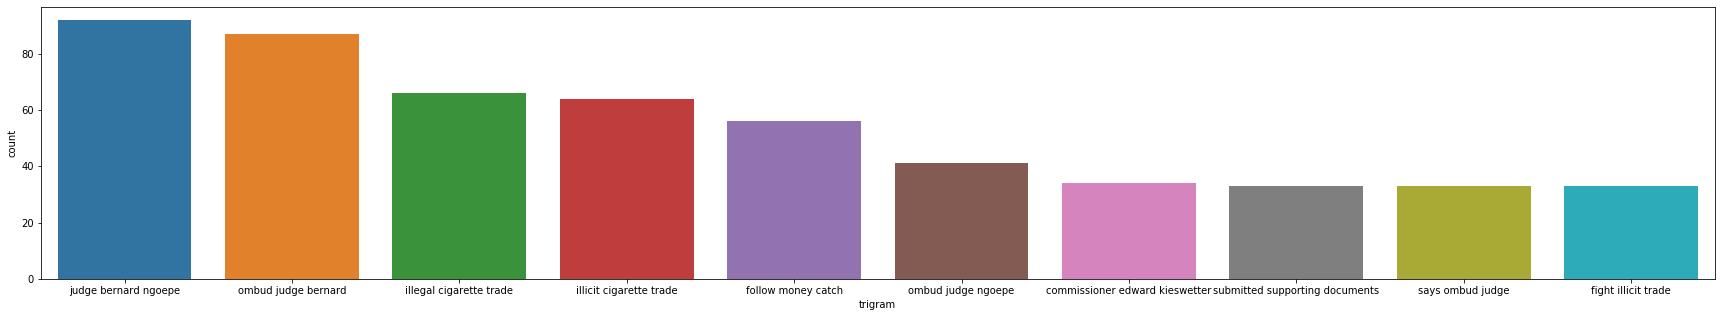
\includegraphics[width=\linewidth]{Tri-gram second second user data.png}
		\caption{Tri-Grams outputs}
		\label{fig:Associated Tri-Gram Outputs}
	    \end{subfigure}
	   \vfill
	 \caption{Comparing Bi-Gram vs. Tr-Grams in Phrase Modelling.}
\end{figure}

Whereas, the bi-grams visualisation for the 2 words which frequently appear together are tax service related on matters taxpayers needed clarity on.

\begin{itemize}
    \item Emerging topics from text analysis
\end{itemize}

The text analysis technique that has been leveraged on to deduce a list of possible topics resulting from overall corpus is the LDA Topic Modelling Technique.  In comparison to other unsupervised topic models algorithms such as the Latent Semantic Indexing (LSI), Hierarchical Dirichlet Process (HDP).  The LDA is more reliable to produce coherent and quality topics when evaluating results with other models as it shows to have better coherence metric values, as shown below.\\

\begin{figure}
      \centering
	    \begin{subfigure}{0.25\linewidth}
		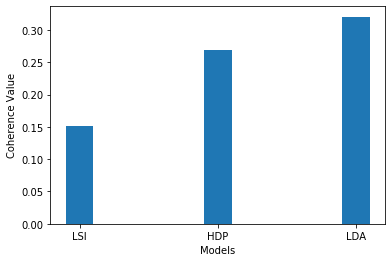
\includegraphics[width=\linewidth]{Evaluate coherence values.png}
		\caption{Coherence values performance }
		\label{fig: Coherence Values}
	   \end{subfigure}
	   \begin{subfigure}{0.25\linewidth}
		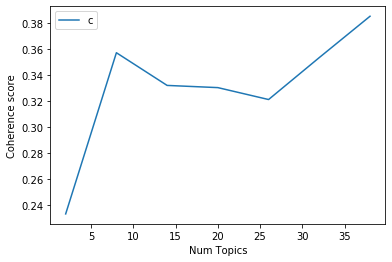
\includegraphics[width=\linewidth]{Number of Topics for the overall data.png}
		\caption{Visual representation of Number of Topics}
		\label{fig:Number of Topics selection}
	    \end{subfigure}
	   \vfill
	 \caption{Comparing topic models coherence values vs  number of topics}
\end{figure}

In order to get the main themes for created topics resulting from the LDA algorithms the process start with the best choice parameters for a finer model by running the CV grid search method to find the best parameters for the LDA.  To initialize  involves feature extraction from the document term matrix of a TF-IDF vector to carry out the topic modelling. The matrix comes with a sparsicity of 0,48 percent following the data processing and removal of stop words, last consideration is the maximum features of 1000.\\
As shown above in fig 9 clearly that the parameter for number of topics =with a value of 10 has a better score for the coherence score of 0.36.\\

Overall results therefore, the base LDA model has the final hyperparameters based on CV Grid search method as follows, the number of topics=10, the learning method for the algorithm updating the assignment of topics to the documents=online, together with the maximum number of iterations to be carried out =10 and the random state = 100.\\
The results are 10 distinct topics despite some topics could share common keywords, it may help to checking for proportion of assigned topics by the model.  In checking the results we can check the proportion of topics that have been assigned to the first document using the lines of code given below.

The table below shows that Topic 10 has the highest proportion

Proportions of topics from the document:\\
\begin{itemize}
    \item Topic  0 :  5.0000000003264145 %\\
\end{itemize}
\begin{itemize}
    \item Topic  1 :  5.000530695799997 %\\
\end{itemize}
\begin{itemize}
    \item Topic  2 :  5.001280907842061 %\\
\end{itemize}
\begin{itemize}
    \item Topic  3 :  5.000000000379809 %\\
\end{itemize}
\begin{itemize}
    \item Topic  4 :  5.0002008679359955 %\\
\end{itemize}
\begin{itemize}
    \item Topic  5 :  5.000000000399167 %\\
\end{itemize}
\begin{itemize}
    \item Topic  6 :  5.000000000336659 %\\
\end{itemize}
\begin{itemize}
    \item Topic  7 :  5.000000000286975 %\\
\end{itemize}
\begin{itemize}
    \item Topic  8 :  5.00028074430452 %\\
\end{itemize}
\begin{itemize}
    \item Topic  9 :  54.9977067823884 %\\
\end{itemize}

For the following 10 topics resulting in the topic modelling LDA technique the results are listed below:

\begin{itemize}
    \item Topic 0: trade report illicit true follow criminals state zuma million reason
\end{itemize}
\begin{itemize}
    \item Topic 1: return working days long audit refund guys returns months year
\end{itemize}
\begin{itemize}
    \item Topic 2: number efiling waiting branch assist submit received today documents response
\end{itemize}
\begin{itemize}
    \item Topic 3: good hope refunds look company file things issue pravin police
\end{itemize}
\begin{itemize}
    \item Topic 4: thank thanks ombud customs exactly believe email address sent compliance
\end{itemize}
\begin{itemize}
    \item Topic 5: unit right commissioner sure start great maybe rogue point minister
\end{itemize}
\begin{itemize}
    \item Topic 6: people problem country like really public question wrong getting white
\end{itemize}
\begin{itemize}
    \item Topic 7: cigarettes paid going paying free taxes read open crime president
\end{itemize}
\begin{itemize}
    \item Topic 8: government illegal corruption business black check court dont evidence years
\end{itemize}
\begin{itemize}
    \item Topic 9: come money stop want details know time need help tell
\end{itemize}

Therefore the topic 10 listed topics from the corpus are listed below as:

When using human judgements to determine the topics are as follows:
\begin{itemize}
    \item Topic 1:  Fight illegal trade activity 
\end{itemize}
\begin{itemize}
    \item Topic 2: long turnaround times post returns submission
\end{itemize}
\begin{itemize}
    \item Topic 3: Minister appointment of commissioner
\end{itemize}
\begin{itemize}
    \item Topic 4:  Appreciatiing tax ombud results
\end{itemize}
\begin{itemize}
    \item Topic 5: Hope for tax refunds appropriateness
\end{itemize}
\begin{itemize}
    \item Topic 6: Minister address rogue unit 
\end{itemize}
\begin{itemize}
    \item Topic 7: Urgent llicit cigarette trade tax crime 
\end{itemize}
\begin{itemize}
    \item Topic 8: Government corruption loosing battle in providing evidence
\end{itemize}
\begin{itemize}
    \item Topic 9:  assistance required case number to query details 
\end{itemize}

Overall the topics discovered through the topic modelling LDA technique realte to the activities for the four years covered. 

\begin{itemize}
    \item Sentiment outputs from text analysis
\end{itemize}

Having explored possible topics from the 4 year engagement discussions, the next is sentiment analysis for overall breakdown engagement of reactions and inputs from users online interaction that can add up emotions from messages with the government department experience over the years covered in the study.  This is to add some quantitative metrics through sentiment analysis in the data exploration analysis.

As messaged add up based on social media use and analysing users comments overtime using a VADER function in python software for a Natural Language Processing (NLP) technique.  
The VADER (Valence Aware Dictionary and sEntiment Reasoner) is a lexicon and rule-based sentiment analysis library of the SentimentIntensityAnalyzer class in Python which returns 4 values, pos, neu, neg and compound.  The compound score is normalised rating of the pos, neu and neg ratings for a single metric value to determine a sentiment. 

The algorithm returns sentiment rating for each tweet for positive, negative and neutral and a compound value to provide a general sentiment of the string.  
While fig 5.14 shows distribution of the normalised compound scores that provides basis for the overall sentiment metric, the actual sentiment scores shows higher neutral sentiments, followed by positive with narrow margin, however the negative sentiment is lowest as shown by Fig 5.15.  At the same time the trend seem to be the same actoss all months of the calendar year depicted in Fig 5.16.\\

\begin{figure}
      \centering
	    \begin{subfigure}{0.25\linewidth}
		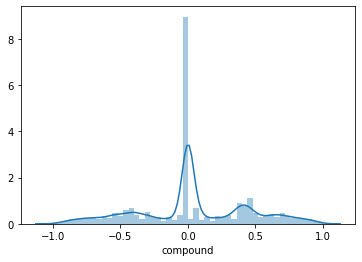
\includegraphics[width=\linewidth]{Sentiment Compound 2.png}
		\caption{Compound results}
		\label{fig:subfig1}
	   \end{subfigure}
	   \begin{subfigure}{0.25\linewidth}
		\includegraphics[width=\linewidth]{Overall Sentiment 2.png}
		\caption{Monthly Sentiments Rating}
		\label{fig:subfig2}
	    \end{subfigure}
	   \vfill
	   \begin{subfigure}{0.25\linewidth}
	   \includegraphics[width=\linewidth]{Overall Sentiments.png}
	   \caption{Overall Sentiment Rating}
	   \label{fig:subfig3}
	   \end{subfigure}
	 \caption{Comparing blue car vs. red car.}
\end{figure}

In all each tweet message has been classified and scored into a sentiment metric of either positive, negative or neutral to get an overview of citizens emotions on their engagements.  It is also possible to observe the sentiments related with the hashtags for the few tweets that have hashtags as shown in Figure and Figure for positive and negative sentiments:\\

\begin{figure}
      \centering
	    \begin{subfigure}{0.25\linewidth}
		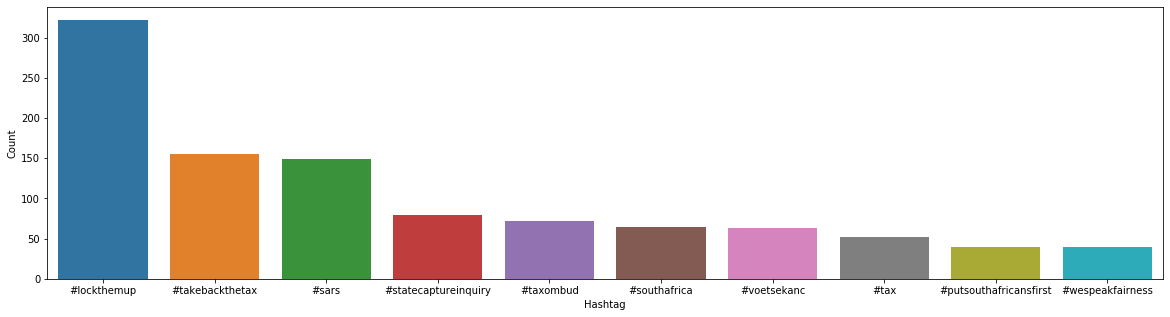
\includegraphics[width=\linewidth]{Sentiments Hashtag Negative.png}
		\caption{Hashtags associated with negative sentiments}
		\label{fig:subfig1}
	   \end{subfigure}
	   \begin{subfigure}{0.25\linewidth}
		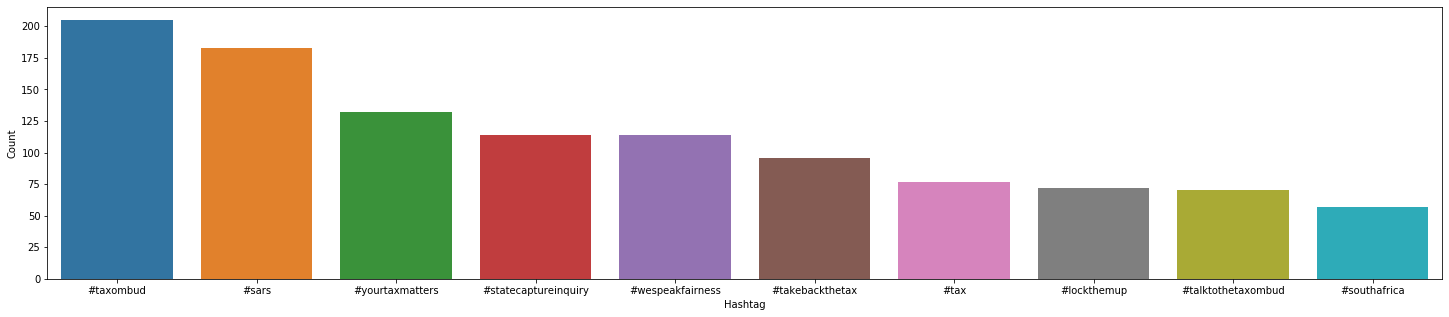
\includegraphics[width=\linewidth]{Hashtag Sentiments Positive.png}
		\caption{Hashtags associated with positive sentiments}
		\label{fig:subfig2}
	    \end{subfigure}
	   \vfill
	 \caption{Comparing blue Negative vs. Positive Sentiment Hashtags.}
\end{figure}

In applying human judgement the possibility of hashtags associated with the sentiments are validated to align\\ 

\subsubsection{Conclusion}

The results of the chapter aim to answer RQ1 abd RQ2 by covering qualitative findings through an exploratory data analysis that has produced results providing insights, understanding including characteristics and behavioural engagements measured between the users, a government and  citizens.\\  Through the ground theory approach for the analysis has revealed results amongst others that users tweets have little usage of hashtags, thus resulting in a hashtag recommendation system to optimise effective use of social media for tweets for the government department under a decade of using twitter.  This chapter is important to give context to the proposed hashtag recommendation solution as a need from the results of user engagements from historical factors.  

\end{document}
\clearpage

\chapter{Conclusions}

\section{Summary of Conclusions}
\label{sec:conclusions:conclusion_summary}

The purpose of this chapter is to summarize the experiment results with findings from the analysis conducted to answer the sub objectives of the study.  In exploring the Twitter data from government the research methodology described in the previous questions covers both qualitative for text mining while this chapter will be quantitative techniques for machine learning algorithms to predict hashtags.

Therefore the chapter is divided according to the following, 1) Exploratory data analysis which has been the main focus of the RQ1, followed by Topic Modelling and Sentiments stemming from the 4 year data to answer RQ1 and RQ2 and lastly, machine learning prediction techniques for hashtag recommendation to answer RQ3.  All in the efforts to answer the research sub-objectives.

\subsection{Summary of Findings}

The study considers a large user community of citizens and government yielding tweets data that has been explored in a study on understanding characteristics and hashtag recommendation techniques. 

\subsubsection{RQ1:Exploratory Data Analysis:}
Present an overview of the descriptive statistics and general insights obtained from the Twitter dataset.
Analyze user engagement metrics, such as the number of tweets, retweets, likes, replies, and followers, to understand user activity and involvement.
Explore temporal patterns and trends in user engagement, identifying peak periods, popular topics, or events that drive higher engagement.\\

"Our study shows that hashtag usage by a user community is very skewed. Very few hashtags enjoy high popularity in tweets and users, while the vast majority of them are used in one tweet or by one user. This observation is consistent with the earlier studies.

\subsubsection{RQ2:}

Having gone through the process of collecting Twitter data, 
with the application of the preprocessing steps applied to the data, such as cleaning, tokenization, removing stop words, handling hashtags/mentions, and any specific considerations for Twitter data.
The processing for removal of noise in the data resulting in the experimental dataset containing 7 887 tweets, total length of the dataset is 761 122 characters with 51 hashtags.  Also some of the interesting characteristics include 104 987 words, 13.33 mean number of words per tweet, Mean length of a tweet is 97.0.\\

We began by discussing the importance of text mining in extracting meaningful information from large volumes of text data. By using techniques such as tokenization, stemming, and sentiment analysis, we were able to process textual data and prepare it for further analysis.

\subsubsction{RQ3:Hashtag Recommendation Prediction}
For the experiment for hashtag recommendation the prediction techniques used both supervised and unsupervised.  To accommodate the supervised models a target label for hashtags tokens has been  created for the experiment.  The majority of the data set was therefore removed, leaving only 11,2 percent of the overall dataset, a small sample.  Explain the process of topic modeling, such as using techniques like Latent Dirichlet Allocation (LDA) to identify latent topics in the Twitter data.
Present the identified topics and their corresponding keywords, along with their prevalence in the dataset.
Discuss the interpretability and coherence of the topics, emphasizing their relevance and representativeness of the Twitter conversations.\\

\textbf{Classification is a supervised learning method that trains a classifier to predict a class label given an instance. While binary classifiers tackle only two categories, multiclass classifiers tackle multiple categories. Hashtag recommendation is commonly tackled as a multi-class classification problem of hashtags [49,52,53,56], where every hashtag is considered as a distinct class label. The intuition of the classification based hashtag recommendation is that the abundance in posts and hashtags equip classifiers with an immense amount of labelled data to learn strong representations [80]. Classification-based hashtag recommendation requires less task-specific assumption and engineering in comparison with topic-based hashtag recommendation [80].
Mention the focus on comparing the performance of topic modeling against supervised techniques (SVM and RF classifiers) for hashtag recommendation.\\}

\subsection{Implications and Recommendations:}
Discuss the implications of the findings for Twitter users, such as the potential for improved content discovery, enhanced user engagement, and more relevant hashtag recommendations.
Highlight the advantages of leveraging topic modeling techniques for hashtag recommendation prediction and its potential benefits for user experience and overall engagement on Twitter.
Provide recommendations for Twitter and its users, such as incorporating topic modeling into hashtag recommendation systems, leveraging the identified topics for content curation, or exploring user-specific topic preferences for personalized recommendations.\\

\subsection{Conclusion:}

Summarize the key findings from the EDA, emphasizing the superiority of topic modeling over supervised techniques for hashtag recommendation prediction.  Highlight the insights gained regarding user engagement and the potential benefits of topic modeling in understanding Twitter conversations.  Conclude with potential future research directions, such as refining topic modeling approaches, incorporating sentiment analysis, or exploring the temporal dynamics of user engagement and topic preferences on Twitter.

The hashtag recommendation system can be useful phenomenon for microblog communication in particular in the context of government communication with citizens within an e-government approach.  Generally, Twitter use has also gained popularity as a communication platform between government with citizens due to availability of internet-data and usage of smart phones devices aiding easy access and use.  However, the amount of Twitter data produced can be overwhelmingly large in terms of volume and scattered bringing limitations of interpretability when not categorized for efficient understanding of topics especially relating to government operational and policy making matters.  The study has shown that 11,65 percent of user tweets does not carry hashtags.  Hence, then this study proposes a personalized hashtag recommendation method type that considers textual content of tweets content only. 

Resulting in an experiment setup consideration of supervised and unsupervised machine learning algorithms for a hashtag recommendation solution to an uncategorised tweets. The supervised learning techniques considered random forest and support vector machines classifiers. Whereas the unsupervised considered topic modelling an Latent Dirichlet Algorithmn.  Of which the based topic model as the best performing to find meaning latenty topics and global hashtags (pyLDAVIS output).  Given a user and a tweet, our method selects the top most similar users and top most similar tweets. Hashtags are then selected from the most similar tweets and users and assigned some ranking scores. Experiment results show that using user preferences and tweet content will give us better recommendation than just using tweet content alone but paying attention the accuracy of the model.

\subsection{Summary of Contributions}

Analysing social media use characteristics and text mining outcomes can be instrumental in understanding its usability, effectiveness and big data prospects.
On the whole, this paper makes a number of contributions to hashtag analysis and recommendation as shown below:
– For the first time, a very large user community and its tweets have been used in a study on hashtag usage and recommendation. We have observed in this dataset that less than 12% of tweets contain hashtags.  The study results indicate effective prediction techniques of up to 5 hashtags at a tweet level of a government tweets and also tax revenue related.  
– The study has developed a hashtag recommendation method that can recommend up to 5 hashtags, considering only the tweet content. 

Percentage of posts that have recommended hashtags in the test set, with a threshold of 0.010 is 72 percent.  This means only 28 percent of tweets could not have a hashtag classification.  Possible attributable characteristics affecting quality of tweets such as mean number of words per tweet of 13.33 words, 
Mean length of a tweet is: 97.0 when maximum is 140 words.  Overall topic coherence evaluation for exploration of results in topic modeling is effectively showing interpretrable topics for the 72 percent cases with hashtags. 

Therefore, the study results show that the unsupervised method for LDA Topic Modelling can achieve hashtags prediction when asked to identify up to 5 new hashtags to users for a tweet.  Due to a small dataset the model comparisons for best performance was only be done for the 2 models using supervised techniques.  The LDA comprised of accuracy score of 0,00 for hashtag recommendation prediction of up to 5 hashtags when compared to the RF and SVM  classification models, with 0,17 and 0,16 respectively.  

\section{Future Work}
%%\label{sec:conclusions:future_work}

Enumerate the future work that you could foresee developing from the work you have done here. Mention areas you could not focus on, or possible extensions to your work. It is a good idea to be thorough, since you increase your chances of being referenced by other researchers who follow up on your work, even if you do not do so yourself. You may consider writing this as a bulleted list, if you mention many aspects.


\clearpage

%%%%%%%%%%%%%%%%%%%%%%%%%%%%%%%%%%%%%%%%%%%%%%%%%
%%%%%%%%%%%%%%%%%%%%%%%%%%%%%%%%%%%%%%%%%%%%%%%%%

\cleardoublepage
\phantomsection

\label{bibliography}
\addcontentsline{toc}{chapter}{Bibliography}
\bibliographystyle{plain}
\bibliography{dissertation}

%%%%%%%%%%%%%%%%%%%%%%%%%%%%%%%%%%%%%%%%%%%%%%%%%
%%%%%%%%%%%%%%%%%%%%%%%%%%%%%%%%%%%%%%%%%%%%%%%%%

\appendix
\directlua{input_all(appendix_includes)}

%%%%%%%%%%%%%%%%%%%%%%%%%%%%%%%%%%%%%%%%%%%%%%%%%
%%%%%%%%%%%%%%%%%%%%%%%%%%%%%%%%%%%%%%%%%%%%%%%%%

\cleardoublepage
\phantomsection
\label{index}
\addcontentsline{toc}{chapter}{Index}
\printindex

%%%%%%%%%%%%%%%%%%%%%%%%%%%%%%%%%%%%%%%%%%%%%%%%%
%%%%%%%%%%%%%%%%%%%%%%%%%%%%%%%%%%%%%%%%%%%%%%%%%













\end{document}
